% spedoc.tex V3.0, 13 May 2010

\documentclass[times]{speauth}

\usepackage{moreverb}
\usepackage{makeidx}  % allows for indexgeneration
\usepackage{graphicx}
\usepackage{subfigure}
\usepackage{amssymb}
\usepackage{amsmath,bm}
%\usepackage[]{algorithm2e}
\usepackage{latexsym}
\usepackage{algorithm} %format of the algorithm
\usepackage{algorithmic} %format of the algorithm
\usepackage{multirow} %multirow for format of table
\usepackage{color}
\usepackage{xcolor}
\usepackage{tabularx}
\renewcommand{\algorithmicrequire}{\textbf{Input:}}
\renewcommand{\algorithmicensure}{\textbf{Output:}}
\newcommand{\KZ}[1]{\textcolor{blue}{(Kenny: #1)}}

%\usepackage[dvips,colorlinks,bookmarksopen,bookmarksnumbered,citecolor=red,urlcolor=red]{hyperref}
\usepackage[colorlinks,bookmarksopen,bookmarksnumbered,citecolor=red,urlcolor=red]{hyperref}


\newcommand\BibTeX{{\rmfamily B\kern-.05em \textsc{i\kern-.025em b}\kern-.08em
T\kern-.1667em\lower.7ex\hbox{E}\kern-.125emX}}

\def\volumeyear{2010}

\begin{document}

\runningheads{Yue Ding et. al.}{}

\title{Exploiting Long- and Short-term Preferences and RFID Trajectories in
Shop Recommendation}

\author{Yue Ding$^1$, Dong Wang$^2$, Guoqiang Li$^2$\corrauth, Daniel W. Sun$^3$, Rajiv Ranjan$^4$,  Xin Xin$^2$, Shiyou Qian$^1$}
\address{\center $^1$ Department of Computer Science and Engineering, Shanghai Jiao Tong University, Shanghai, China\\
$^2$School of Software, Shanghai Jiao Tong University, Shanghai, China\\
$^3$Data61, CSIRO, Australia\\
$^4$School of Computing Science, Newcastle University, United Kingdom
}
\corraddr{School of Software, Shanghai Jiao Tong University, Shanghai 200240, China \\ li.g@sjtu.edu.cn}

\begin{abstract}
Shop recommendation in large shopping malls is useful in the 
mobile internet era. With the maturity of indoor positioning technology, 
customers' indoor trajectories can be captured by RFID readers, 
which provides a new way to analyze customers' potential preferences. 
In this paper, we design three methods for the top-N shop recommendation 
problem. The first method is an improved matrix factorization(MF) 
method fusing estimated prior customer preference matrix which is 
constructed by Session-based Temporal Graph(STG) computing. 
The second method is a Bayesian Personalized Ranking (BPR) method based on 
the first method. The third method is by tensor decomposition combined with STG.Besides, we exploit customer history RFID trajectory information to 
find customers' frequent paths and revise predicted rating values to 
improve recommendation accuracy. Our methods are effective in modeling 
customers' temporal dynamics. At the same time our approach considers
repeated recommendation of the same shop by designing rating update rules. 
The test dataset is formed by \emph{JoyCity} customer behavior records. 
JoyCity is a large-scale modern shopping center in downtown Shanghai, 
China.  The results show that our approaches are effective and 
outperform previous state-of-the-art approaches.


\end{abstract}

\keywords{ Matrix Factorization, Tensor, BPR, RFID Trajectories, Recommendation}

\maketitle              % typeset the title of the contribution


\section{Introduction}

\KZ{Change all occurrences of ``consumption'' or ``consume'' to ``transaction''
or ``purchase''.}
Large online stores such as Amazon.com have successfully deployed 
recommender systems to make recommendations according to customers' potential 
interests. While online stores attract more and more customers, 
traditional physical shopping malls provides spaces for people to
shop, relax and socialize in the real world and hence continue to exist and
thrive in every part of the world. 
%are still irreplaceable, different with traditional local shopping malls, 
%a modern shopping center is not only a place for shopping, 
%it also integrates other functions like dining, leisure and entertainment. 
Recommender system can be useful to both online and offline shopping experience.
The goal of the recommendation is to suggest new or less popular (a.k.a. long
tail) items to users~ \cite{Yin2012VLDBChallengingTheLongTail}. 
Most online item recommendation tends to suggest unknown items and 
rarely considers items already purchased by the same user. Shop recommendation,
on the other hand, needs to take into account that a shop contains 
hundreds of items and a customer may visit a specific shop repeatedly 
at different times. We consider this specialized problem as 
repetitive recommendation. When designing shop recommendation algorithms, 
both customers' temporal dynamic behaviors and the repetitive 
recommendation problem should be considered to make more accurate and 
reasonable recommendation.

Traditional neighborhood-based methods for collaborative filtering aim to find similar users or similar items and make recommendations \cite{ref29}. The drawbacks of neighborhood approaches are inefficiency in sparse and cold start 
situations. Latent factor model (LFM) is now a popular approach in recommender 
systems. The LFM approach presents the primitive matrix by product of 
two low rank matrices, connecting users and items by latent factors. 
LFM possesses good scalability.
In the shopping mall scenario, many factors may influence customers' 
consumption such as periodic shopping seasons, discounts and promotions, 
special events, etc. Apparently, customers' preferences are changing, 
which makes it difficult to model customers' temporal dynamics. 
The temporal dynamics is a challenging topic in recommender systems. 
The existing approaches have low prediction accuracy. In this paper, 
we design a set of three approaches that all aim to process temporal 
dynamics for shop recommendation.
We capture customers' long- and short- term preferences by computing a 
Session-based Temporal Graph(STG)\cite{ref03}, all customers' preferences 
in a new time window can be estimated as a preference bias matrix. 
For the first approach, we fuse the bias matrix into matrix factorization, 
called MF-STG. For the second approach, we adopt a Bayesian Personalized 
Ranking (BPR)\cite{ref25bpr} method on explicit feedback by MF-STG, 
called MF-STG-BPR. For the third approach, we apply a three dimensional 
tensor decomposition approach that utilize STG bias matrix as prior 
estimation, called Tensor-STG. MF-STG and Tensor-STG handle rating 
prediction or ranking tasks, MF-STG-BPR processes ranking task only. 
Tensor-STG fully considers temporal dynamics on higher dimensions.

In order to make more accurate prediction, we build context-aware rating 
update rules. The context-aware information includes two parts, 
customers' past RFID(radio frequency identification devices) trajectory data 
and customers' past purchases. On the one hand we exploit customer 
RFID trajectories to mine customers most frequented paths and hence
their potential shops of interest, then increase the predicted rating 
values accordingly. RFID technology has been successfully applied in 
many areas. Large shopping malls which have deployed RFID readers can 
capture registered members information and record indoor trajectories. 
The trajectory information implicitly reflect customer preferences. 
On the other hand, we design rating update rules based on customer's past 
transactions. We consider a special problem that may occur in shop 
recommendation: should we recommend a shop which the customer has patrionized
before? The intuition is that for a shop that a customer has patronized, 
if the predicted rating is lower than his individual average rating, 
the predicted rating should be adjusted higher, otherwise, it should 
be adjusted lower.

Our proposed approaches perform well on temporal dynamics, all customers' 
long- and short-term preferences are estimated in the form of matrix which 
is calculated by STG. The flexible matrix factorization and tensor 
decomposition method nicely fuse this estimated preference matrix and 
achieve good performance. 
The BPR method that utilizes the estimated preference matrix further improves 
the ranking result. The Tensor-STG aims to make rating prediction in a 
new time window on three dimensional tensor structure, 
which better explains the result.
The experimental results show that our approaches outperform the 
state-of-the-art algorithms, and our methods are applicable to 
shop recommendation. The key contributions of this paper are summarized as
follows:

\begin{enumerate}
\item Matrix factorization and Tensor decomposition fused customer long- 
and short-term preferences;
\item Bayesian Personalized Ranking(BPR) and RFID trajectories enhances the
recommendation accuracy;
\item Rating update rules fully considers the repetitive recommendation.
\end{enumerate}

The rest of the paper is organized as follows. Section 2 discusses related work. Section 3 describes algorithms. Section 4 presents experiment result and Section 5 concludes the paper.



\section{Related Work}
Matrix Factorization (MF) model is the most successful approach with good 
scalability in rating prediction. Given observed matrix R of size $p \times q$, 
R can be approximated by two low-dimensional matrices $M$ and $D$, 
where $M$ is of size $p \times k$, $D$ is of size $k \times q $. 
Koren et al. \cite{ref05} surveys MF related methods for recommender system 
and proposes modified MF models by adding baseline biases, 
input sources for cold start problem, temporal dynamics and inputs with 
varying confidence levels respectively. Andriy et al. \cite{ref02} present 
the Probabilistic Matrix Factorization (PMF) model with view of probability 
and extend PMF to include an adaptive prior for model parameters.
Josef et al.\cite{ref04} extend PMF from normal distribution assumption 
to a flexible framework with general probabilistic distributions.
Yu et al.\cite{ref07} apply PMF and build explicit and implicit feedback 
data for IP-TV recommendation.
Qian et al.\cite{ref08} propose a personalized recommendation algorithm 
based on PMF that combines personal interest, interpersonal interest 
similarity and interpersonal influence. \cite{3review06} proposes 
user-service rating prediction approach by exploring social users�� 
rating behaviors. Ahn et al.\cite{3review02} propose a scalable distributed 
Bayesian MF algorithm using stochastic gradient MCMC.

Modeling temporal dynamics is challenging since user's preference is drifting and items' popularity is also changing. Ding et al.\cite{ref12} propose an algorithm which calculates time weight for items. Time-window and instance-decay approaches may cause the problem of losing much signal, thus debasing prediction accuracy. Koren \cite{ref01} proposes time changing baseline predictors to model temporal behavior. Graph computing and tensor analysis \cite{ref14}\cite{ref15} perform well on modeling temporal dynamics. Liang \cite{ref03} designs a long- and short-term performance fused graph framework. The approach divides time into different sessions and measures users' preference by leveraging user-item connection and session-item connection. Tensor model represents data with high dimensions. CANDECOMP/PARAFAC(CP) decomposition and Tucker decomposition \cite{ref19} for higher-order tensors have wide applications in data mining \cite{ref23}, computer vision \cite{ref24} and graph analysis \cite{ref22}.

Newly emerging location-based social networks (LBSNs) such as 
Facebook Places have experienced very fast growth with the rapid 
development of Web 2.0, location acquisition and wireless communication 
technologies. In LBSNs, users can post their physical locations 
with geo-tagged information in the form of 'check-in' and 
share their visiting experiences and tips for points of interest 
(POI)\cite{3review08}. LBSNs provide a new platform for us to understand 
user preferences and bring opportunities and challenges for 
recommender systems to solve the cold start as well as 
sparsity problems \cite{3review07}. 
POI recommendation has become an important way to help people 
discover interesting places \cite{3review09}\cite{3review10}\cite{3review11}. 
Wang et al. \cite{WeiqingKDD2015Geo} propose a geographical sparse 
additive generative model (Geo-SAGE) for spatial item recommendation. 
\cite{HongzhiTOIS2014LCARS} and \cite{ref18} propose a location-content-aware 
recommender system to provide venues and events recommendation considering 
users' both personal interests and local preferences. 
Yin et al. \cite{HongzhiACMMM2015Joint} \cite{HongzhiCIKM2015Joint} 
propose a unified probabilistic generative model to analyze the joint 
effect on users�� decision-making for POIs by mining the semantic, 
temporal and spatial patterns of users check-in activities. 
\cite{HongzhiTOIS2016Joint} proposes Topic-Region Model (TRM) and 
extends it to an online learning model for real-time POI recommendation.

\cite{3review01} proposes a real-time product recommendation system 
called METIS that detects user's purchase intents from their microblogs 
and makes product recommendation by extracting and matching user and 
item demographic information. \cite{3review03} studies the geographical 
neighbourhood influence for business rating prediction.
\cite{3review04} proposes  Connoisseurs over Consumers (COC) model 
to make real-time recommendation in communities.
Wang et al.\cite{3review05} propose collaborative deep learning model 
users non-i.i.d input.

Different from LBSN based POI recommendation that puts emphasis 
on exploiting users shared experiences and tips for recommendation, 
our proposed approaches for indoor shop recommendation focus on 
predicting customers evolving preferences. 
POI recommendations utilize social information, geographical information 
and user ``check-in'' information to improve prediction accuracy; 
we use indoor RFID trajectories and design rating update rules to 
improve prediction accuracy. The fusion of matrix factorization and STG 
takes the convenient advantage of MF for its flexibility and the 
advantage of STG for its good performance on processing temporal dynamics. 
The result of STG as a bias matrix for MF can overcome the disadvantage of 
STG in which the determination of time window size may affect 
recommendation accuracy and computational complexity. 
The MF-STG method can provide more stable and flexible solution without 
regardless of the time window size selection in STG. 
The adoption of BPR method helps to get more accurate ranking result. 
The Tensor-STG method is different from the existing methods that are 
good at restoring the tensor while difficult to perform ranking task; 
we utilize the STG result matrix as pre-estimated customer preferences 
in a new time window in the tensor structure. 
To formulize the task, for a set of customers $U$, a set of transaction $R$, 
a set of shops $I$, a set of RFID trajectories  $T$, 
we predict customer ratings $R_{ui}$ utilizing MF-STG, MF-STG-BPR 
and Tensor-STG. We evaluate our result by leave-one-out Hit Rate 
(HR) and Average Reciprocal Hit-Rank (ARHR).


\section{The Approaches}
In this section, we present our approaches. Section 3.1 describes the architecture for shop recommendation. Section 3.2 introduces the consumption-rating mapping method that converts customer past purchases to a rating value. 
Section 3.3 to Section 3.5 present the proposed methods, namely MF-STG, 
MF-STG-BPR and Tensor-STG respectively. 
Section 3.6 describes (1)how to exploit RFID trajectories to mine 
customer's potential preferences and improve recommendation accuracy; 
(2)The rating update rules that adjust predicted ratings where customer 
has made transactions.

\subsection{The Architecture of Proposed Shop Recommendation}
Figure 1 illustrates the architecture of shop recommendation. The raw data is composed of two parts: customer transaction data and RFID trajectory data. 
The customer transaction data comes from POS terminals while the RFID 
trajectory data comes from the RFID readers. The transaction data is 
aggregated into a user-shop matrix, and then the transaction values are 
converted to a rating matrix. We propose three algorithms, all of which 
can make top-N recommendation. 
\KZ{Consider simplify the following as it repeats parts of the
intro.} The common ground of these three algorithms 
is that we adopt a Session-based Temporal Graph (STG) which estimates 
prior user preference matrix. The MF-STG approach fused the STG result matrix 
as a bias term into matrix factorization. MF-STG-BPR utilizes the 
estimated matrix and adopts a Bayesian Personalized Ranking (BPR) method. 
The Tensor-STG approach construct a three dimensional tensor 
(customer-shop-time) model, we use the STG result matrix as 
initial prediction slice and apply nonnegative Tucker decomposition. 
The differences among these approaches are: (1) MF-STG and Tensor-STG can deal with rating prediction or ranking tasks, MF-STG-BRP can only cope with ranking task. (2) Tensor-STG models temporal dynamics on higher dimension.

On the other hand, for customer RFID trajectory data, we sort the customer's visited areas by timestamp, then we obtain the customer's most frequent 
visited areas by applying APRIORI algorithm, before finally obtaining
the list of the customer's frequently visited shops. 
The information of customer's frequently visited shops is 
converted to increase the value of predicted ratings, 
which can be considered as positive feedback. 
We also design rating update rules which may increase or decrease the 
value of predicted ratings depending on the customer's average rating. 
The rating update rules are only applied to the shops where the customer 
has made a purchase.

\begin{figure}[h]
  \centering
  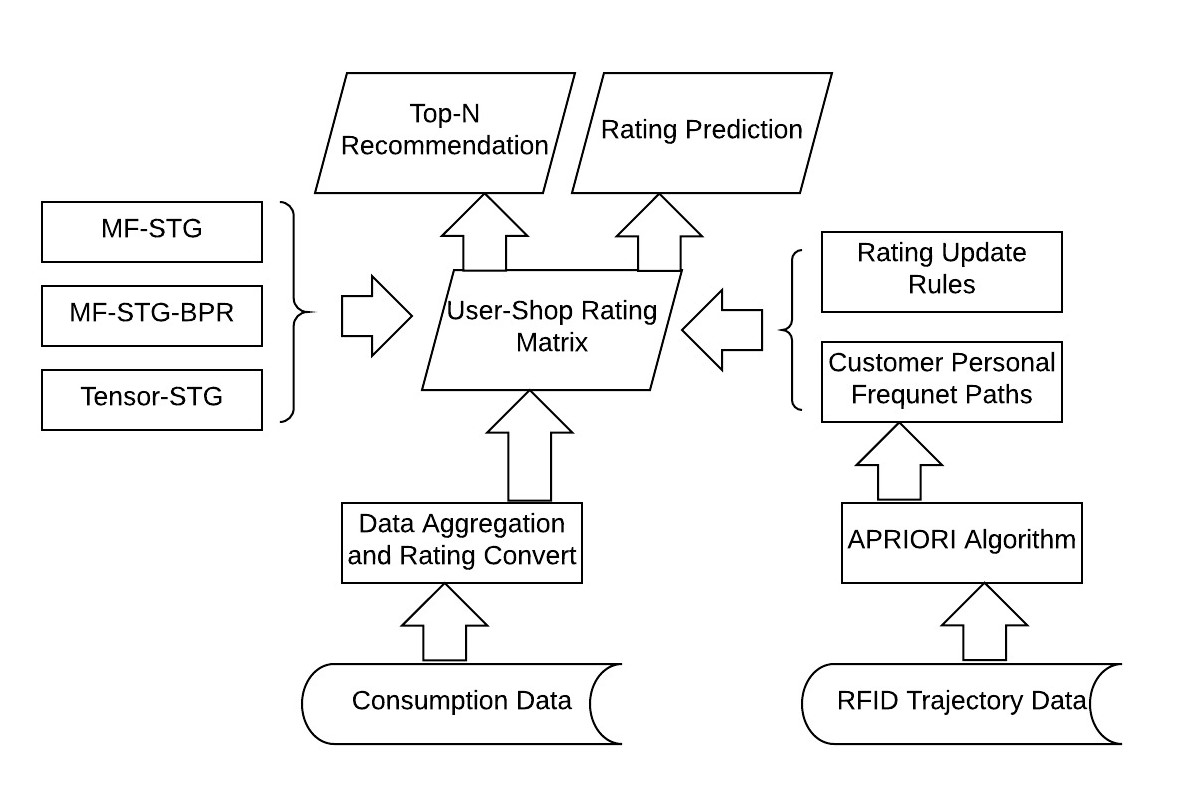
\includegraphics[scale=0.6]{framework}
  \caption{The Architecture of Shop Recommendation}\label{The Architecture of Shop Recommendation}
\end{figure}


\subsection{Generate Rating Matrix}
Let $U$ be the user set, $I$ be the item set. In the shopping scenario, an item is a shop which contains a variety of products. Our algorithms aim to recommend shops to customers that they may have interest. Customer transaction data 
can implicitly reflect their preference. We use a mapping function to 
convert customers historical transaction data to a real rating value 
and construct a customer-shop rating matrix.

Let $R$ of size $|U|\times |I|$ be the rating matrix, $R_{ui}$ 
represents customer $u$'s rating to shop $i$, $R_{ui}\in (0,5)$ 
and $R_{ui} =5$ indicates the highest preference while $R_{ui} =0$ 
indicates no preference to a given item. 
The formulations are described as follows.

\begin{equation}
\begin{array}{lcl}
  R_{u\!i} & = & F(S_{u\!i})\\
\end{array}
\end{equation}

\begin{equation}
\begin{array}{lcl}
  S_{u\!i} & = & \sum_{t\in Time} A_t(u\!i)\\
\end{array}
\end{equation}

\begin{equation}
\begin{array}{lcl}
  F(x) & = &10\times \left( \left(\frac{1}{1+exp\left( -\frac{1}{1000}x\right)}\right)-0.5\right)
\end{array}
\end{equation}

Where $A_t(u\!i)$ is the amount customer $u$ paid at shop $i$ at time $t$ 
and $u\in U$, $i\in I$. $S_{ui}$ represents customer $u$'s total consumption on shop $i$.  The mapping function converts any transaction value 
to rating interval (0, 5).

\subsection{MF-STG}
For temporal dynamics in recommender systems, a customer's preference is 
drifting and an item's popularity is changing over time. 
To deal with this challenging issue, Koren\cite{ref01} builds linear baseline predictors to capture user's preference, however the result shows that the improvement is limited. Although Koren's approach can be fused with other factorization or neighborhood methods, the model complexity increases and more parameters need to be trained. Liang Xiang\cite{ref03}'s model of Session-based Temporal Graph(STG) fuses user's long- and short-term preference over time. The Injected Preference Fusion(IPF) algorithm can perform top $N$ recommendation. But STG has its disadvantage. When creating session nodes, the determination of time window size has obvious influence on recommendation accuracy and computational complexity. The smaller size of time window achieves better accuracy while increasing complexity. There is no flexible way to determine the optimal size. 

\subsubsection{Result Matrix Construction.}
For our proposed MF-STG method, we refer STG framework to construct a similar graphic model for customer preference prediction. But instead of making top $N$ recommendation from STG computing, we construct a user-item matrix as pre-estimate customer preference bias matrix. Thus, no matter how time window size changes in STG, the MF method can obtain a reasonable result.

STG model breaks time dimension into different sessions instead of treating time as a universal dimension that is shared by all users. Figure 2 illustrates a simple example of STG model which is a directed bipartite graph $G(U,S,I,E,\omega)$. Set $U$ denotes user nodes, set $S$ denotes sessions, set $I$ denotes item nodes, set $E$ denotes edges of graph and set $\omega$ denotes weights with different non-negative values for edges. User nodes are linked with items that are viewed by each user, which represents users' long-term preference. Session nodes are linked with items that users viewed at time $T$, which represents users' short-term preference at time $T$.

\begin{figure}[h]
\centering
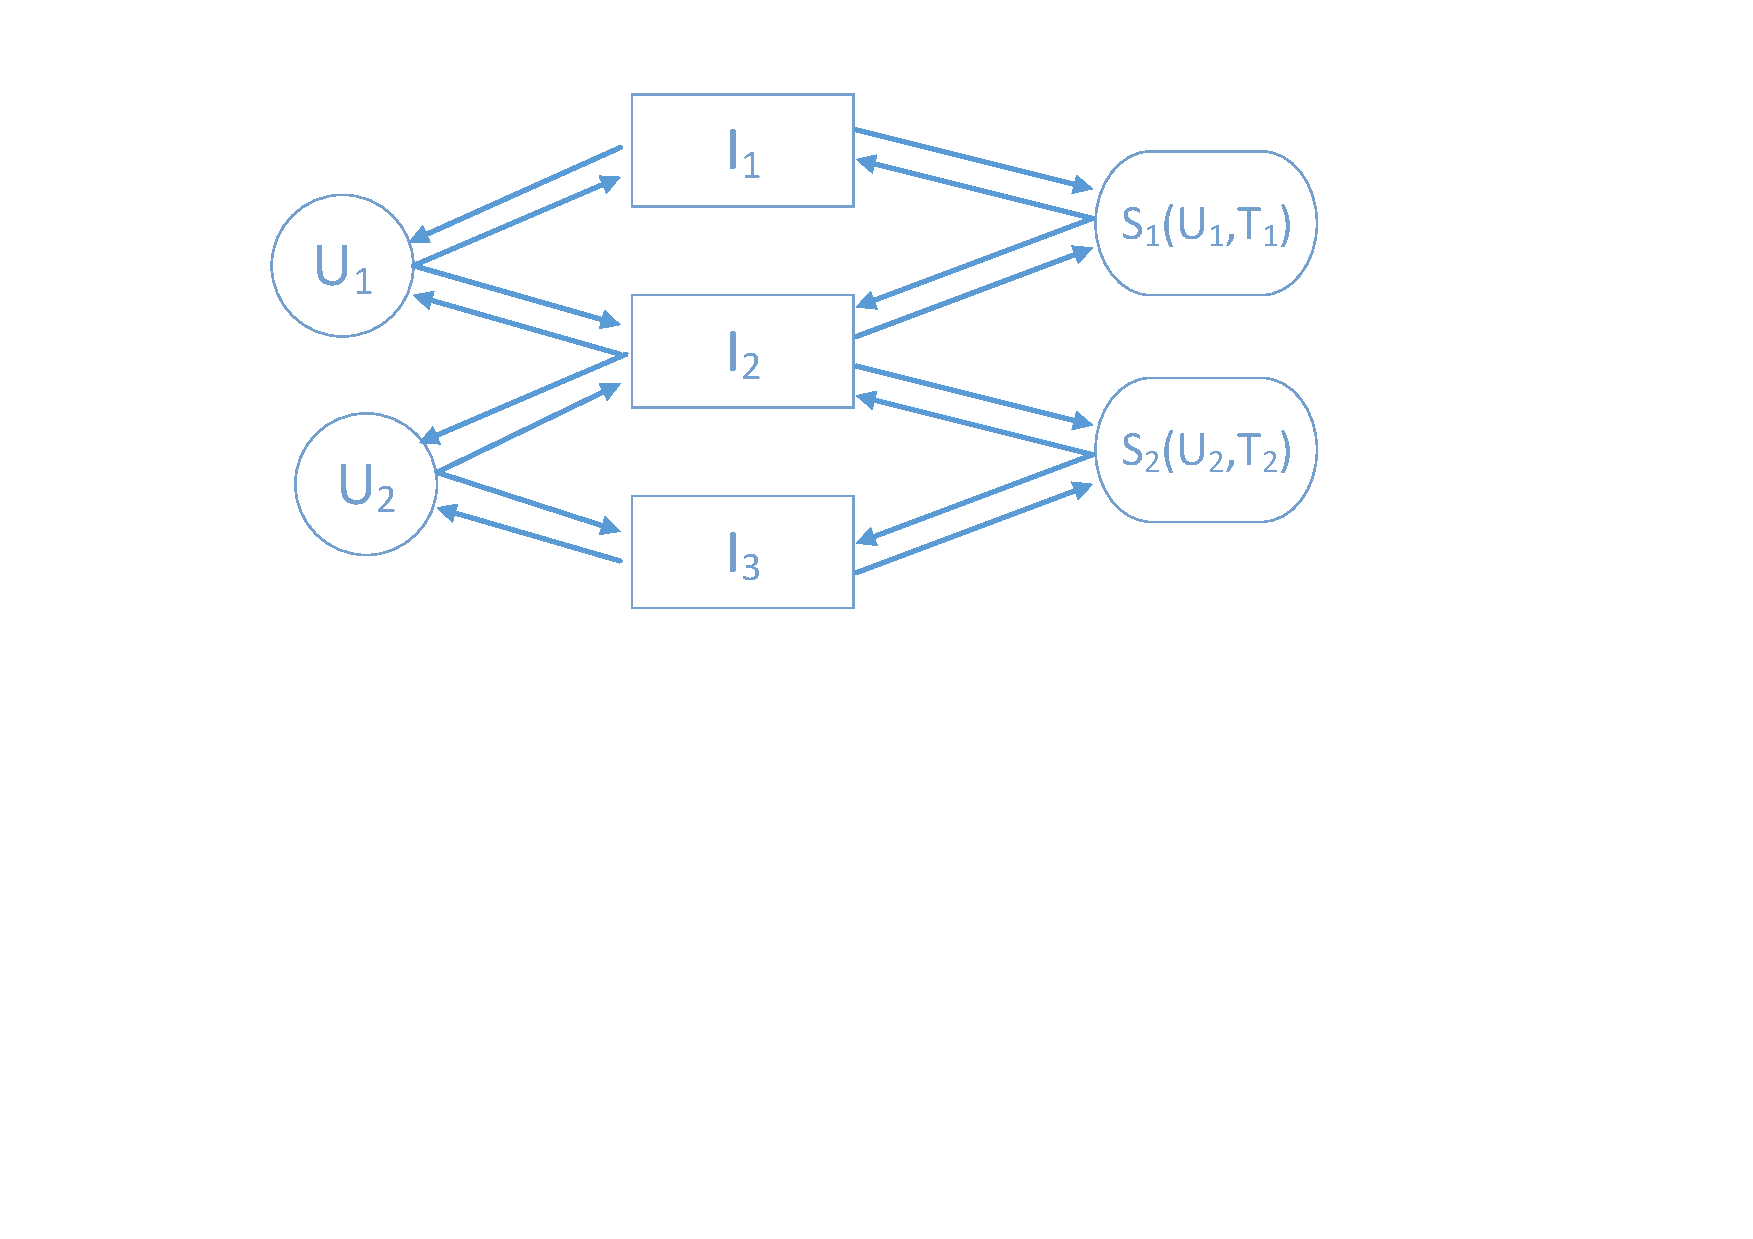
\includegraphics[scale=0.3]{STG}
\caption{A simple example of STG}
\label{figure03}
\end{figure}

The weight value $\omega$ between different nodes $v$ and $v'$ is defined as:

\begin{equation}
\omega(v,v')=\left\{
\begin{array} {ll}
1, \quad if  & v\in U\cup S , v' \in I\\
\eta_u , \quad if  &   v\in I, v' \in U \\
\eta_s , \quad if  &   v\in I, v' \in S
\end{array}
\right.
\end{equation}

Equation (4) defines $\omega$ in different cases. If $v$ is from set $U$ or $S$ and $v'$ is from set $I$, the weight value is 1. If $v$ is from set $I$ and $v'$ is from set $U$, the weight value is $\eta_u$. If $v$ is from set $I$ and $v'$ is from set $S$, the weight value is $\eta_s$. Set source node $v_0\in \{ v_u,v_{ut}\}$ and end node $v_n\in \{ v_i\}$ where $v_u$ is from $U$, we see
that the source point could be a user node or a session node, the end point is an item node.
Let $PATH$ be the path of nodes between the source node $v_0$ and 
an unknown item node $v_n$, i.e., $PATH=$\{ $v_0,v_1,......v_n$ \}. 
The preference value from $v_0$ to $v_n$ is defined in Equation (5).

\begin{equation}
\Phi(PATH)=\prod\nolimits_{\nu_{k\in {PATH}, 0\leq k <n}}\Omega(v_k, v_{k+1})\Upsilon(v_0),
\end{equation}
where $\Upsilon(v_0)$ is defined as follows,

\begin{equation}
\Upsilon(v_0)=\left\{
\begin{array}{ll}
w , &    v_0=v_u\\
1-w , & \quad v_0 = v_{u\!t}
\end{array}
\right.
\end{equation}

$w$ is the parameter that controls the weight from different sources. $\Omega(v_k, v_{k+1})$ is defined as follows,

\begin{equation}
\Omega(v_k, v_{k+1}) = \left\{
\begin{array}{ll}
  \frac{1}{|out(v_k)|^\rho}, & \quad v_k \in U\cup S, v_{k+1}\in I \\
  \left(\frac{\eta}{\eta|out(v_k)\cap U|+|out(v_k)\cap S|}\right)^{\rho}, & \quad v_k\in I, v_{k+1}\in U\\
  \left(\frac{1}{\eta|out(v_k)\cap U|+|out(v_k)\cap S|}\right)^{\rho}, & \quad v_k\in I, v_{k+1}\in S
\end{array}
\right.
\end{equation}

$\Omega(v_k, v_{k+1})$ calculates preference from node $v_k$ to its next 
node $v_{k+1}$. \emph{out}($v_k$) is the out-degree of node $v_k$. The larger \emph{out}($v_k$) is, the less incoming preference $v_{k+1}$ will have. Parameter $\rho$ ranges from zero to one and $\rho$ controls \emph{out}($v_k$)'s impact exponentially. Parameter $\eta$ = $\eta_u$ / $\eta_s$ and the definition of $\eta_u$ and $\eta_s$ is in Equation (4). To simplify the solving process, only shortest paths with its length of three from user or session node to unrated item is considered.
Define $pre_{u\!i}$ as user $u$'s estimated preference on unrated item $i$, the final calculation of $pre_{u\!i}$ is defined by Equation (8).

\begin{equation}
pre_{u\!i} =\sum_{pre\in\mathcal{PATH}(u,i)}\Phi(PATH)
\end{equation}


\subsubsection{MF-STG Learning Algorithm. }
We use low rank matrices $P$ of size $p \times k$ and $Q$ of size $k \times q$ to approximate observed rating matrix $R$ of size $p \times q$, where $k$ is the latent factor. $p_u$ is the $u^{th}$ row vector in $P$ and $q_i$ is the $i^{th}$ column vector in $Q$. We generate pre-estimate $bias$ matrix from STG result. Thus the prediction of unknown item $i$ by user $u$ is formed as

\begin{equation}
r'_{u\!i} =\tau\cdot bias_{ui} + p_u q_i,
\end{equation}
where $\tau$ is the weight factor of $bias_{ui}$. The objective function is formed as

\begin{equation}
\begin{array}{rl}
\Psi = \min\limits_{p^{\star},q^{\star}\!} &\sum_{(u,i)\in k}\frac{1}{2}(r_{u\!i}-\tau\cdot bias_{ui}- p_uq_i)^2\\& + \frac{\beta}{2}\left(||p_u||_F^{2}+||q_i||_F^{2}\right),
\end{array}
\end{equation}
where
$\frac{\beta}{2}\left(||p_u||_F^{2}+||q_i||_F^{2}\right)$
is the regularized constraint and $||\cdot||_F$ is the $Frobenius$ Norm for preventing overfitting. We train parameters by applying a stochastic gradient descent algorithm.

\begin{equation}
\frac{\partial \Psi}{\partial p_u}=-e_{u\!i}\cdot q_i +\beta\cdot p_u
\end{equation}
\begin{equation}
\frac{\partial \Psi}{\partial q_i}=-e_{u\!i}\cdot p_u +\beta\cdot q_i
\end{equation}
Here $e_{ui}$ is the error between observed value $r_{ui}$ and estimated value $r'_{ui}$.
\begin{equation}
e_{ui} = r_{ui} - r'_{ui} = r_{ui} - \tau\cdot bias_{ui} - p_u q_i
\end{equation}
The update rules for parameters $p_u$ and $q_i$ are
\begin{equation}
p_u \leftarrow p_u +\alpha(e_{u\!i}\cdot q_i -\beta \cdot p_u)
\end{equation}
\begin{equation}
q_i \leftarrow q_i +\alpha(e_{u\!i}\cdot p_u -\beta \cdot q_i),
\end{equation}
where $\alpha$ is the learning rate to control convergence.

\subsection{MF-STG-BPR}
In this section, we introduce how to conduct a Bayesian Personalized Ranking (BPR) on the MF-STG method. BPR is a generic approach for personalized ranking problem \cite{ref25bpr}. It is the maximum posterior estimator derived from a Bayesian analysis. Define explicit feedback $S_E \subseteq U \times I$, where $U$ is the user set and $I$ is the item set. Define $I_u^+$ and $U_i^+$ as follows:
\begin{equation}
I_u^+ = \{i \subseteq I : (u,i)\in S_E \}
\end{equation}
\begin{equation}
U_i^+ = \{u \subseteq U : (u,i)\in S_E \}
\end{equation}
$I_u^+$ is the item set rated by user $u$ and $U_i^+$ is the user set that has rated on item $i$. Define set $D_{S_E} = U \times I \times I$ by:
\begin{equation}
D_{S_E} =\{(u,i,j)|i \in I_u^+ \wedge j \in I\backslash I_u^+ \}
\end{equation}
$(u,i,j)\in D_{S_E}$ denotes user $u$ may have potential interest on item $i \in I_u^+$ over item $j \in {I \backslash I_u^+}$. Maximize the following posterior probability by Equation (19) to get all users' personalized ranking for all items.
\begin{equation}
p(\Theta | >_u) \propto p(>_u | \Theta)p(\Theta)
\end{equation}
$>_u$ is the short for $i >_u j$ which indicates that for each item pair $(i,j)$, user $u$ may prefer item $i$ to item $j$. $\Theta$ is the parameter space. In MF-STG-BPR, $\Theta$ consists of low rank matrices $P$ and $Q$. 
Assuming all users are independent of each other, each pair of items $(i,j)$ is independent of each other, the likelihood function $p(>_u | \Theta)$ can be 
presented as:
\begin{equation}
\prod_{u\in U} p(>_u | \Theta) = \prod_{(u,i,j)\in U\times I\times I }  p(i >_u j|\Theta)^{\delta ((u,i,j)\in D_{S_E})} \cdot (1-p(i >_u j|\Theta))^{\delta ((u,i,j)\notin D_{S_E}},
\end{equation}
where $\delta$ is the indicator function:

$$ \delta (b)=
\begin{cases}
1& \text{if b is true}\\
0& \text{else}
\end{cases}$$
From definition of $p(i >_u j)$ , the following properties can be deduced,
\begin{equation}
\forall i,j \in I : i\neq j \Rightarrow i >_u j \vee j >_u i
\end{equation}
\begin{equation}
\forall i,j \in I :  i >_u j \vee j >_u i \Rightarrow i = j
\end{equation}
Then the likelihood function $p(>_u | \Theta)$ can be simplified to
\begin{equation}
\prod_{u \in U} p(>_u|\Theta) = \prod_{(u,i,j)\in D_{S_E}} p(i >_u j|\Theta)
\end{equation}
In order to get user's personalized ranking result, define $\hat{x}_{uij}$ as user individual probability that user $u$ prefers item $i$ to item $j$ , then we can deduce that
\begin{equation}
p(i >_u j|\Theta) = \sigma (\hat{x}_{uij}(\Theta)),
\end{equation}
where function $\sigma$ is:
\begin{equation}
\sigma (x) = \frac{1}{1 + e^{-x}}
\end{equation}
For equation(23), assume $p(\Theta)$ is subject to a normal distribution with zero mean and covariance matrix $\Sigma_{\Theta}$.
\begin{equation}
p(\Theta) \sim N(0,\Sigma_{\Theta})
\end{equation}
To simplify hyperparamters, we set $\Sigma_{\Theta}=\lambda_{\Theta}I$. 
The maximum posterior estimator of BPR, called BPR-OPT, can be derived as:
\begin{displaymath}
\begin{aligned}
BPR-OPT = \ & ln \ p(\Theta|>_u) \\
        = \ & ln \ p(>_u|\Theta)p(\Theta) \\
        = \ & ln \prod_{u,i,j \in D_{S_E}} \sigma(\hat{x}_{uij})p(\Theta) \\
        = \ & \sum_{u,i,j \in D_{S_E}} \ ln \sigma(\hat{x}_{uij}) + ln \ p(\Theta) \\
        = \ & \sum_{u,i,j \in D_{S_E}} \ ln \sigma(\hat{x}_{uij}) - \lambda_\Theta||\Theta||^2, 
\end{aligned}
\end{displaymath}
where $\lambda_\Theta$ is regularization parameter set. The update rules of hyperparameters $\Theta$ can be derived as equation (27) by applying stochastic gradient descent.
\begin{equation}
\Theta \leftarrow \Theta + \alpha \left( \frac{e^{\hat{x}_{uij}}}{1 + e^{\hat{x}_{uij}}} \cdot \frac{\partial}{\partial \Theta} \hat{x}_{uij} + \lambda_{\Theta} \Theta \right)
\end{equation}

In MF-STG-BPR, we define $\hat{x}_{uij}(\theta)$ = ($\hat{x}_{ui} - \hat{x}_{uj} | \theta = (p_u, q_i, q_j))$, where $p_u$ represents the $u^{th}$ row vector in low rank matrix $P$, the size of $P$ is $p \times k$. $q_i$ and $q_j$ represent the $i^{th}$ and $j^{th}$ column vector in low rank matrix $Q$, the size of $Q$ is $k \times q$. Set $q_i$ contains items that user $u$ has rated and set $q_j$ contains items that user $u$ has not rated. Obviously, $q_i \cup q_j = Q$. We can derive $\hat{x}_{uij}$ as following:
\begin{equation}
\hat{x}_{uij} = (\tau \cdot bias_{ui} + p_u q_i)-(\tau \cdot bias_{uj} + p_u q_j)
\end{equation}
Then the gradient with respect to parameters $\theta$ for MF-STG-BPR model is:
\begin{equation}
\frac{\partial}{\partial \theta} \hat{x}_{uij} = \left\{
\begin{array}{ll}
  q_i - q_j \quad & if \quad \theta = p_u \\
  p_u & if \quad \theta = q_i\\
  -p_u & if \quad \theta = q_j
\end{array}
\right.
\end{equation}
Accordingly, we set three regularization factors: $\lambda_{p_u}$ for user feature matrix, $\lambda_{q_i}$ for user rated updates and $\lambda_{q_j}$ for user unrated updates. We give the detailed learning algorithm of MF-STG-BPR. Once we get the estimated parameters $p_u$, $q_i$ and $q_j$, the rating prediction of user $u$ on item $v$ is calculated by:
\begin{equation}
r'_{uv} = \tau \cdot bias_{uv} + p_u q_v
\end{equation}

The learning algorithm of MF-STG-BPR is shown in $Algorithm 1$.

\begin{algorithm}[h] %Algorithm begin
\caption{The Learning Algorithm of MF-STG-BPR} %Algorithm title
\label{algorithm MF-STG-BPR} %Label
\begin{algorithmic}[1] %control to use ':'
\REQUIRE Rating matrix $R$, STG result $bias_{ui}$%Input:
\ENSURE $p_u, q_i, q_j$ %Output
\STATE BEGIN
\STATE INITIAL:
\STATE $\alpha \leftarrow $ learning rate
\STATE $F \leftarrow$ Number of latent features
\STATE $P \leftarrow Normal Distribution \sim (0,1)/10$
\STATE $Q \leftarrow Normal Distribution \sim (0,1)/10$
\STATE $S_z \leftarrow$ number of sampled zeros
\STATE $S_{nz} \leftarrow$ number of sampled non-zeros
\STATE $\lambda_{p_u},\lambda_{q_i},\lambda_{q_j} \leftarrow$ regularization factor
% while-loop
\WHILE{steps $<$ MaxSteps}
\FORALL{$u \in U$}
\FORALL{$i \in random(R_u^+ (S_{nz}))$}
\STATE $Z \leftarrow SampleZeros(S_z) $
\FORALL{$j \in Z$}
\STATE $\hat{x}_{uij} = (\tau \cdot bias_{ui} + p_u q_i) - (\tau \cdot bias_{uj} + p_u q_j)$
\STATE $p_u= p_u + \alpha \left( \frac{e^{\hat{x}_{uij}}}{1 + e^{\hat{x}_{uij}}} \cdot \frac{\partial}{\partial \Theta} \hat{x}_{uij} \cdot (q_i - q_j)+ \lambda_{p_u} p_u \right)$
\STATE $q_i= q_i + \alpha \left( \frac{e^{\hat{x}_{uij}}}{1 + e^{\hat{x}_{uij}}} \cdot \frac{\partial}{\partial \Theta} \hat{x}_{uij} \cdot p_u + \lambda_{q_i} q_i \right)$
\STATE $q_j= q_j + \alpha \left( \frac{e^{\hat{x}_{uij}}}{1 + e^{\hat{x}_{uij}}} \cdot \frac{\partial}{\partial \Theta} \hat{x}_{uij} \cdot (-p_u) + \lambda_{q_j} q_j \right)$
\ENDFOR
\ENDFOR
\ENDFOR
\ENDWHILE
\STATE RETURN $p_u, q_i, q_j$
\STATE END
\end{algorithmic}
\end{algorithm}

\subsection{Tensor-STG}
A tensor is an $N$-dimensional array. The number of a tensor's dimension is known as a tensor's order or modes. A tensor with one dimension is a vector and with two dimensions is a matrix. A tensor is a higher-order tensor if it has three or higher dimensions. The advantage of tensor model is that it can nicely represent high dimensional data without breaking its eigen structure. A tensor can be structured by different slices. A tensor's horizontal slices, lateral slices and frontal slices can be presented by $\bm{X_{i::}}$, $\bm{X_{:j:}}$ and $\bm{X_{::k}}$ respectively.

Tucker decomposition is a high-order Principal Component Analysis (PCA) 
approach. A tensor can be decomposed into a \emph{core tensor} and 
factor matrices along each mode. Figure 3 illustrates Tucker decomposition 
of a three-way tensor $\chi$.
%\begin{equation}
%\bm{\chi} \approx \bm{\varrho} \times_1 \bm{A} \times_2 \bm{B} \times_3 \bm{C}
%\end{equation}
Here $\bm{\chi}\in\mathbb{R}^{I \times J \times K}$, $I$,$J$ and $K$ are integers that represent the indices of tensor $\chi$. For $i=1,2...,I, j=1,2...,J, k=1,2...,K$, the element $(i,j,k)$ of tensor $\chi$ is denoted by $x_{ijk}$. $\bm{\varrho}\in\mathbb{R}^{P \times Q \times R}$ is the \emph{core tensor}, factor matrices $\bm{A}\in\mathbb{R}^{I \times P}$, $\bm{B}\in\mathbb{R}^{J \times Q}$ and $\bm{C}\in\mathbb{R}^{K \times R}$ are principal components in each mode and they are normally orthogonal. The elementwise of restored $\chi$ is computer as,
\begin{equation}
x'_{ijk} \approx \sum_{p=1}^P \sum_{q=1}^Q \sum_{r=1}^R g_{pqr} a_{ip} b_{jq} c_{kr}
\end{equation}
An alternating proximal gradient (APG) method is applied for solving nonnegative tucker decomposition\cite{nonnegativeTucker}.

\begin{figure}
  \centering
  % Requires \usepackage{graphicx}
  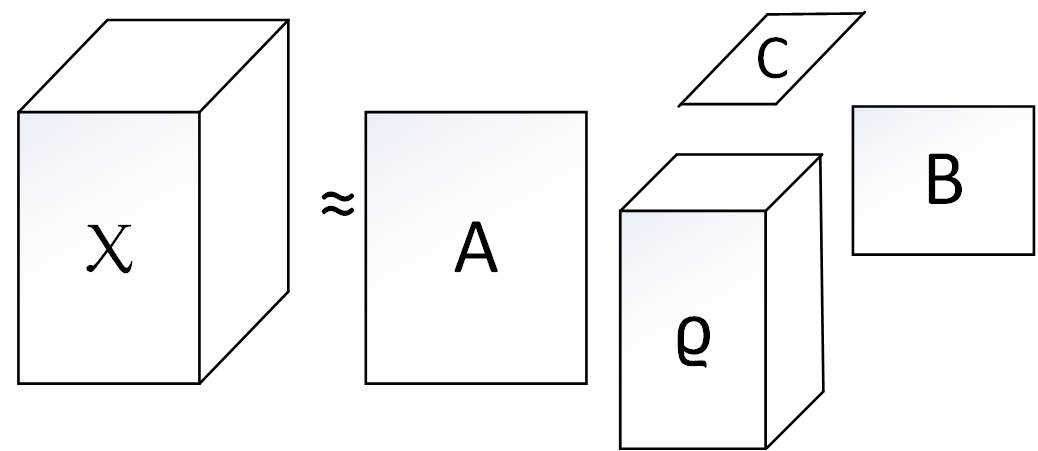
\includegraphics[scale=0.3]{tucker}\\
  \caption{Tuck Decomposition of a Three-way Array}\label{Tuck Decomposition of a Three-way Array}
\end{figure}

%\subsubsection{Rating Prediction Calculating Procedure.}
We apply following steps in Tensor-STG approach:

\emph{Step 1.} Partition the training data sets with fixed time intervals.

\emph{Step 2.} Construct a $Customer-Shop-Time$ three dimensional tensor $\chi$ which is composed of slices $\chi_{::t_1}$, $\chi_{::t_2}$,......,$\chi_{::t_{prediction}}$.

\emph{Step 2.} Adopt STG result as pre-estimate matrix for $\chi_{::t_{prediction}}$.

\emph{Step 3.} Run nonnegative tucker decomposition on observed tensor and get core tensor and other factor matrices.

\emph{Step 4.} The elements of restored tensor can be calculated by equation (31).

Different from the MF-STG and MF-STG-BPR approach in which the rating 
prediction is made on a two dimensional matrix, Tensor-STG fully takes 
into account of temporal dynamics. For shop recommendation, 
for example, if customer $u$ has made a transaction in shop $i$ at
different times $t_1$ and $t_2$, its shopping behavior can be reflected by 
the tensor model, while the two dimensional matrix models fail to do that. 
The rating prediction by the tensor model has better explanation, 
but the drawback is the sparsity of higher order tensors.

\subsection{Rating Update Rules Using Context-ware }
To further improve recommendation accuracy, we adopt two methods using customer context-aware information to adjust predicted ratings. 
There are two types of context-aware information: customer past RFID
trajectories and customer past purchases. To formulate the task, 
we define \{$r'$\} as follows,
\begin{equation}
 \{r'\} =\{I_{u\!k}\vartheta r'_{u\!k}\}\cup \{I_{u\!j}\varpi R(r'_{u\!j})\} \cup  \{r_{u\!l}'\},
\end{equation}
where $I_{uj}$ and $I_{uk}$ are indicator functions.
The set $r'_{uk}$ consists of shops mined from customer's personal most
frequent paths. Parameter $\vartheta$ is the weight factor. 
We divide customer RFID trajectory data by days and mine most frequent paths 
using the $APRIORI$ Algorithm. Figure 4 describes an example of 
mining a customer's maximum frequent visited areas(given support=50\%).
\begin{figure}
  \centering
  % Requires \usepackage{graphicx}
  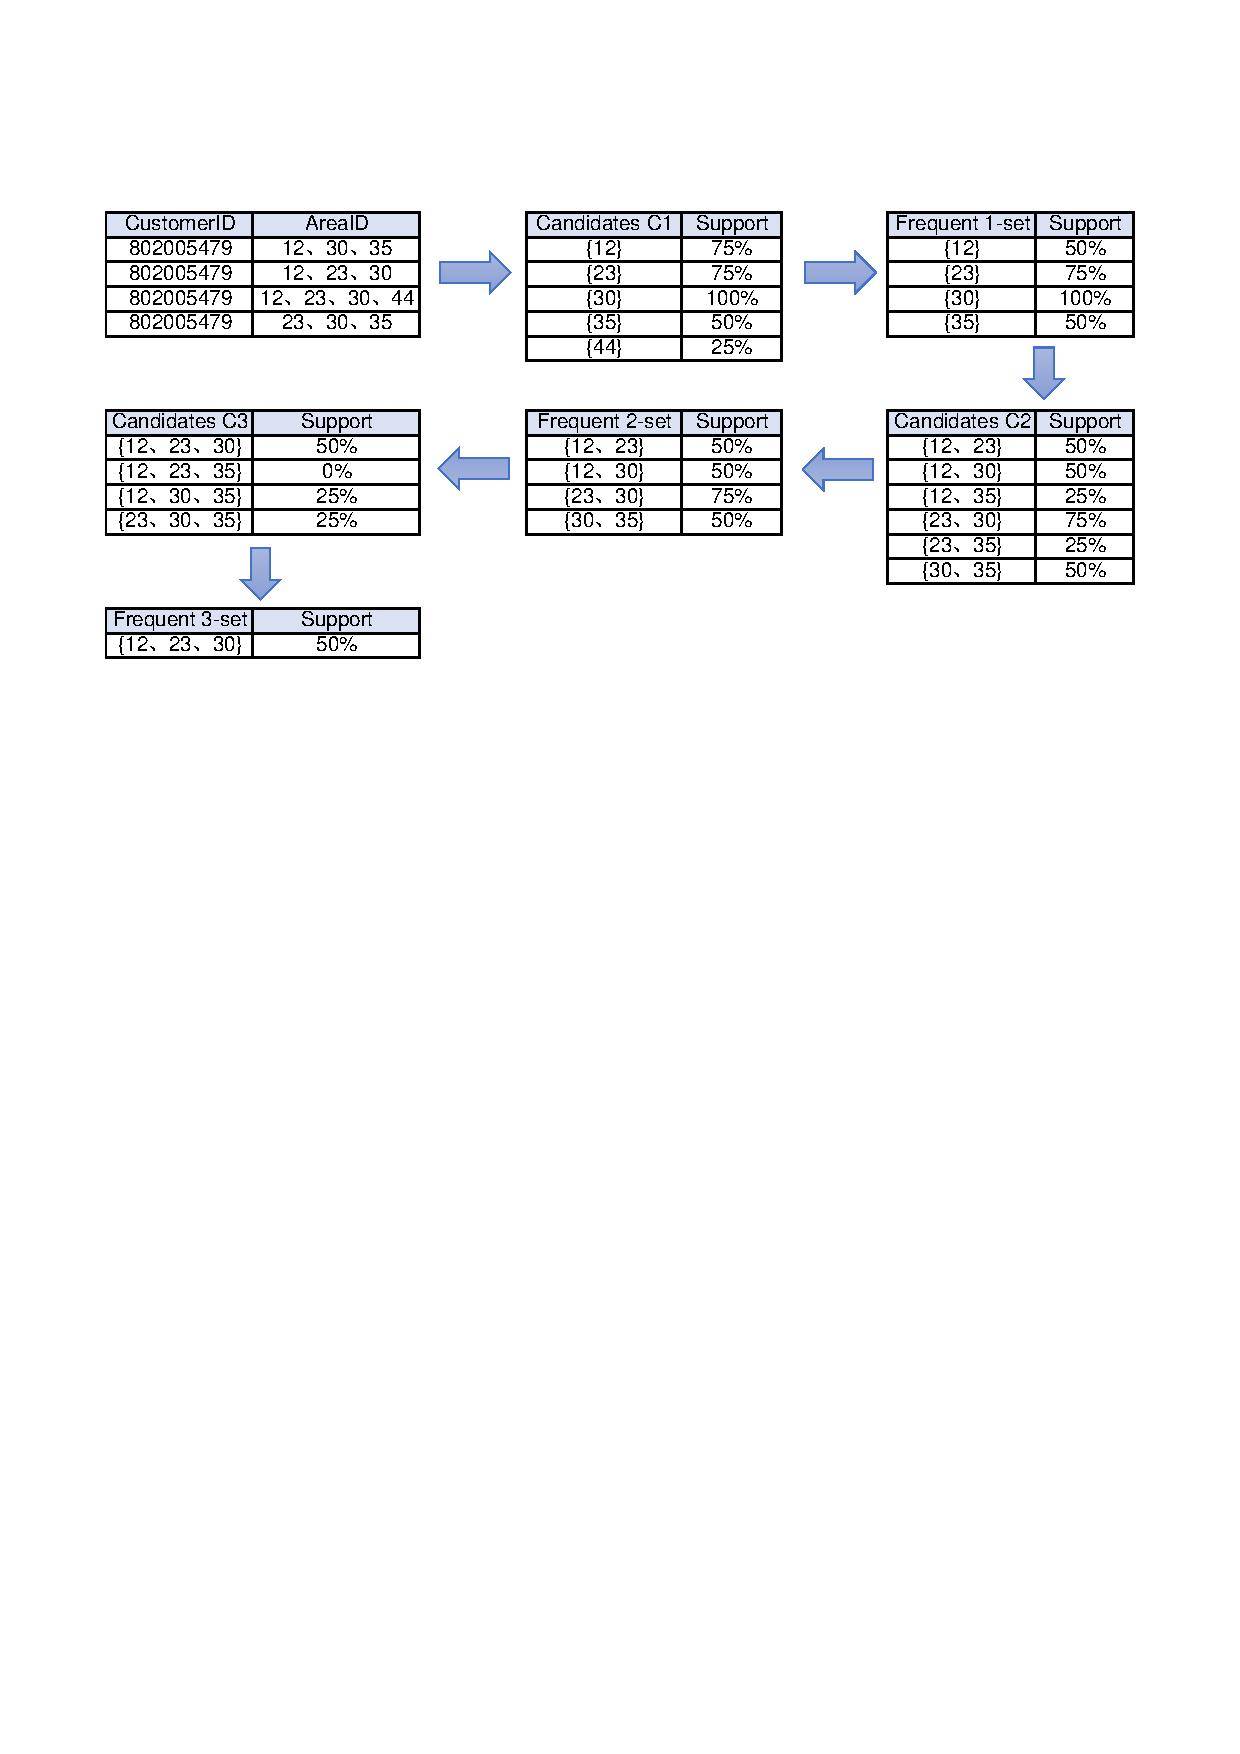
\includegraphics[scale=0.8]{Apriori}\\
  \caption{An Example of Mining a Customer's Maximum Frequent Visited Areas}\label{An example of mining a customer's maximum frequent visited areas}
\end{figure}
The intuition of exploiting RFID trajectories is that the areas frequently
visited by a customer implicitly reflect their interests. 
Accordingly, the predicted ratings for shops near these areas 
should be adjusted higher.

$r'_{uj}$ consists of shops where customer $u$ has made purchases. 
Parameter $\varpi$ is a weight factor. The update function $R(r'_{uj})$ 
is defined in equation (33). $\kappa$ and $\xi$ are output weight factors 
and $\mu$ is the value of average customer rating.
The intuition of designing the rating update rule is that the repetitive 
recommendation should be taken into account for shop recommendation. 
Consider the situation that if a customer has purchased three times in 
a shoe store in the past five months, should we recommend this shoe store 
again? The customer may have lasting interest in the shoe store and patronize
the shoe shop again, but it's inappropriate to recommend the shoe store all 
the time. The customer's average rating $\mu$ is used to measure whether 
the visited shop deserves to be recommended once again. 
If the predicted rating value $r'_{uj}$ is smaller than $\mu$, 
then $r'_{uj}$ should be adjusted higher to make possible repetitive 
recommendation. Otherwise, $r'_{uj}$ should be adjusted lower to deal with 
the situation that the customer may have drifted their interests and 
does not want to pay in this store in the near future. 
The set $r'_{ul}$ contains shops whose rating values are not revised.

\begin{equation}
R(r'_{u\!j})=r'_{u\!j}+\kappa \cdot sign(\mu-r'_{u\!j})\cdot |\mu-r'_{u\!j}|^{\xi}
\end{equation}

\subsection{Complexity Analysis}
In STG, $|E|$ is the total number of edges, $|U|$ is the total number of users, the complexity of user-item bipartite graph is $O(|E|\cdot |U|)$, considering the unfixed number of session-item edges, assuming the number of session-item 
edges is $k$ times larger than the user-item edges, and the total complexity 
of STG is thus $O(k \cdot |E|\cdot |U|)$. For the MF method, let 
$|U|$ be the total number of users, $|I|$ be the total number of items, 
$|F|$ be the feature number of two low rank matrices. In the worst situation in each iteration, the complexity is $O(|U|\cdot|F|+|I|\cdot|F|)$.
For the BPR method, assume we sample $S_{rated}$ number of rated items 
and $S_{unrated}$ number of unrated items for user $u$. 
For the worst situation in each iteration, the complexity of BPR 
in each iteration is $O(|U|\cdot|I|\cdot S_{rated} \cdot|F|+|U|\cdot|I|\cdot  S_{unrated} \cdot|F|)$.
For tucker tensor decomposition, the original tensor is 
$\bm{\chi}\in\mathbb{R}^{I \times J \times K}$, the core tensor $\bm{\varrho}\in\mathbb{R}^{P \times Q \times R}$ factor matrices are $\bm{A}\in\mathbb{R}^{I \times P}$, $\bm{B}\in\mathbb{R}^{J \times Q}$ and $\bm{C}\in\mathbb{R}^{K \times R}$. In each iteration, all the elements in $A,B,C$ and $\varrho$ are updated, the complexity of tucker decomposition in each iteration is hence
$O(|I|\cdot|P|+|J|\cdot|Q|+|K|\cdot|R|+|P|\cdot|Q|\cdot|R|)$.

\section{Evaluation}
In the following, we briefly describe the dataset, the evaluation
metric and the baselines, and present some comparative results.

\subsection{Data Set}
The dataset comes from a large-scale Shanghai shopping call named
\emph{Joycity} which has deployed a RFID system in all indoor space. 
Registered members who carry a membership card can be tracked by the 
RFID readers. 
%Our test dataset is a small part of the whole data. 
The test dataset contains customer RFID trajectories records and 
customer historical transaction records spanning 16 consecutive months. 
The total number of customers is 300, the total number of shops is 280. There are 2019 consumption records and the total amount of customer consumption is 1,826,028 RMB. If the consumption records are aggregated into a customer-shop matrix, the number of converted ratings is 1309, the sparsity is 1.56\%. The RFID trajectory data contains 150,858 records. Table I describes the sample data of customers' consumption records. Table II describes the sample data of RFID trajectories. The sample interval is 0.001 second by RFID readers.

\begin{table}
\centering
\caption{Sample of Customer Consumption Record}
\begin{tabular}{|c|c|c|c|} \hline
 ShopID     &CustomerID   &TimeStamp                &Amount\\ \hline
\ 5F1501    &802000007    &2012-1-18 15:30:45       &2654  \\ \hline
\ 3F1701    &802000007    &2012-3-19 11:28:32       &344  \\ \hline
\ 1F0201    &802016410    &2011-1-16 17:04:09       &4988  \\ \hline
\end{tabular}
\end{table}

\begin{table}
\centering
\caption{Sample of RFID Trajectory}
\begin{tabular}{|c|c|c|c|} \hline
 CustomerID  &ReaderID      &RangeID    &Timestamp\\ \hline
\ 802016700  &191           &103        &2011-03-02 14:46:38.347  \\ \hline
\ 802016700  &14            &4          &2011-03-02 14:47:02.720 \\ \hline
\ 802016700  &23            &13         &2011-03-02 14:51:20.760  \\ \hline
\end{tabular}
\end{table}

\subsection{Evaluation Method and Metrics.}
We adopt 5-time Leave-One-Out cross validation(LOOCV) \cite{ref26SLIM}to evaluate the performance of our proposed methods, the result is the average value. In each run, the dataset is separated into a training set and a validation set. The validation set is formed by randomly selecting one of the non-zero ratings of each user. We use the rest of data as training set to train the model. For each user, a top- N ranked list of recommended items is generated, the recommendation quality is measured by the Hit Rate (HR) and the Average Reciprocal Hit-Rank (ARHR). The definition of HR and ARHR is described as follows,
\begin{equation*}
HR = \frac{\#hits}{\#users} ,
\end{equation*}

\begin{equation*}
ARHR = \frac{1}{\#users} \sum_{i=1}^{\#hits} \frac{1}{p_i} ,
\end{equation*}

where $\#users$ represents the total number of users, $\#hits$ represents the number of users that the recommended items in his $size-N$ recommendation list are hit in validation set. $p_i$ represents the position of item in ranked recommendation list. Higher HR value means higher recommendation quality. ARHR can be considered as a weighted viewpoint in HR.

\subsection{Baseline Algorithms.}
We compare MF-STG, MF-STG-BPR and Tensor-STG with the following baseline algorithms.

\textbf{$UserKNN_{cos}$}: User-based $K-Nearest Neighbors$ using cosine similarity.

\textbf{$ItemKNN_{cos}$}: Item-based $K-Nearest Neighbors$ using cosine similarity.

\textbf{$SVD++$}: A matrix factorization model, rating prediction is composed of several bias parts, SVD++ model also utilizes users' implicit/explicit feedbacks.

\textbf{$STG$}\cite{ref03}: Session-based temporal graph algorithm which models users�� long-term and short-term preferences over time.

\textbf{$BPRMF$}\cite{ref25bpr}: A BPR learning model applied on base matrix factorization.

\textbf{$SLIM$}\cite{ref26SLIM}: Sparse linear methods for Top-N recommendation. SLIM constructs a sparse aggregation coefficient matrix $W$. Prediction is made by aggregating user/item rating matrix and $W$ with $\ell_1 - norm$ and $\ell_2 - norm$ regularization.

\textbf{$FISM_{rmse}$}\cite{ref27FISM}: Item-based Top-N recommendation, which learns item-item similarity matrix as the product of two low rank latent factor matrices.

\textbf{$BPTF$}\cite{BPTF}: Bayesian Probabilistic Tensor Factorization approach using Markov Chain Monte Carlo.

\subsection{Performance Comparison}
Table III describes performance of our proposed approaches and other baseline algorithms. All the methods are evaluated by $Top 5$ and $Top 10$ recommendations. For $UserKNN_{cos}$ and $ItemKNN_{cos}$, $Par1$ represents the number of $k$. For $SVD++$, parameters are the number of latent factors and the regularization factor. For $STG$, parameters are $\rho$, $w$ and $\eta$. For $BPRMF$ and $MF-STG-BPR$, parameters are regularization factors $\lambda_{P_u}$, $\lambda_{Q_i}$ and $\lambda_{Q_j}$. For $SLIM$, parameters are regularization factors for $\ell-1 norm$ and $\ell-2 norm$. For $FISM_{rmse}$, parameters are the number of latent factors and the regularization factor. For $BPTF$, parameters are the feature dimension and the number of samples. For $MF-STG$, the parameter is the regularization factor $\beta$. For Tensor-STG, parameters are the maximum number of  iterations and the tolerance for relative change of function value.
For methods of $SVD++$, $BPRMF$, $SLIM$, $FISM_{rmse}$, $BPTF$, $MF-STG$ and $MF-STG-BPR$, the learning rate is set as 0.001. We use a grid search to find the most suitable parameter. The search space is from 0 to 1 and the increment is 0.1. For $UserKNN$ and $ItemKNN$, the number of $k$ is searched from 10 to 100 and the increment is 10. For the number of latent factors in $SVD++$ and $FISM_{rmse}$ is searched from 10 to 100 and the increment is 10.
\begin{table}[h!]
  \centering
  \caption{Baseline Algorithm Comparison.}
  \label{tab:table2}
  \begin{tabularx}{\textwidth}{@{\extracolsep{\fill}}ccccccccc}
    Methods@Top10 & Par1 & Par2 & Par3 & HR@5 & ARHR@5 & HR@10 & ARHR@10\\
    \hline
    $UserKNN_{cos}$         & 20    & -     & -     & 0.2344 & 0.0992 & 0.2969 & 0.1081\\
    $ItemKNN_{cos}$         & 50    & -     & -     & 0.1016 & 0.0389 & 0.2188 & 0.0536\\
    $SVD++$                 & 10    & 0.2   & -     & 0.0698 & 0.0284 & 0.1085 & 0.0333\\
    $STG$                   & 0.5   & 0.5   & 0.7   & 0.3130 & 0.2177 & 0.4275 & 0.2336\\
    $BPRMF$                 & 0.8   & 0.6   & 0.5   & 0.1406 & 0.0753 & 0.2656 & 0.0913\\
    $SLIM$                  & 0.1   & 0.1   & -     & 0.1221 & 0.0646 & 0.2443 & 0.0803\\
    $FISM_{rmse}$           & 20    & 0.6   &       & 0.2248 & 0.1355 & 0.3256 & 0.1496\\
    $BPTF$                  & 20    & 30     & -    & 0.0846 & 0.0541 & 0.1308 & 0.0534\\
    $\textbf{MF-STG}$       & 0.9   & -     & -     & 0.3462 & 0.2368 & 0.4692 & 0.2538\\
    $\textbf{MF-STG-BPR}$   & 0.7   & 0.6   & 0.7   &\textbf{0.3846} &\textbf{0.2499} &\textbf{0.4988} &\textbf{0.2648}\\
    $\textbf{Tensor-STG}$   & 500   & 1e-4     & -     & 0.2077 & 0.1290 & 0.4012 & 0.1504\\
  \end{tabularx}
\end{table}

The result shows the proposed approaches perform better than baseline algorithms, MF-STG-BPR achieves the best HR and ARHR result on top-5 and top-10 recommendation. We notice that $UserKNN$ performs much better than $ItemKNN$ method, in the shopping mall scenario, users' shopping behavior may directly affect their companions. While users' preference on a specific shop $i$ may imply the exclusion to other similar shops of $i$, so $ItemKNN$ does not perform well. So does $SLIM$ which uses an "item-item similarity co-efficient matrix". We also notice that Tensor-STG doesn't perform as well as MF-STG and MF-STG-BPR. We investigate it and find that the advantage of Tensor-STG is to predict customers' future ratings based on their past ratings. Since the leave-one-out HR and ARHR evaluation method randomly take one non-zero rating from the dataset as the validation set, the training set and the validation set are not strictly time evolved, thus decreases prediction accuracy. We provide another set of test to support this. We reorganize the data that evolves over time, we take first 80\% of the data as the training set and rest 20\% as the validation set. We adopt commonly used $Recall$ and $Precision$ rate as metrics. The definition of $Recall$ and $Precision$ rate are as follows,

\[
Recall =\frac{|\text{PredictionSet}\cap \text{ReferenceSet}|}{|\text{ReferenceSet}|}
\]

\[
Precision =\frac{|\text{PredictionSet}\cap \text{ReferenceSet}|}{|\text{PredictionSet}|}
\]

The $Recall$ rate reflects the portion of correct predicted results in the validation set. The $Precision$ rate reflects the correct rate of predicted results. Figure 5 illustrates the comparision of $Recall$ and $Precision$ rate of MF-STG, MF-STG-BPR and Tensor-STG. Tensor-STG achieves the best recall value of 0.1124 and 0.2202 for $top-5$ and $top-10$ recommendation respectively, and the best precision value of 0.1241 and 0.1215 for $top-5$ and $top-10$ recommendation respectively. Tensor-STG outperforms MF-STG and MF-STG-BPR. The results show that Tensor-STG can make more accurate prediction given time evolving dataset, and at the same time, it is more sensitive to the dataset.

\begin{figure}[h]
  \centering
  % Requires \usepackage{graphicx}
  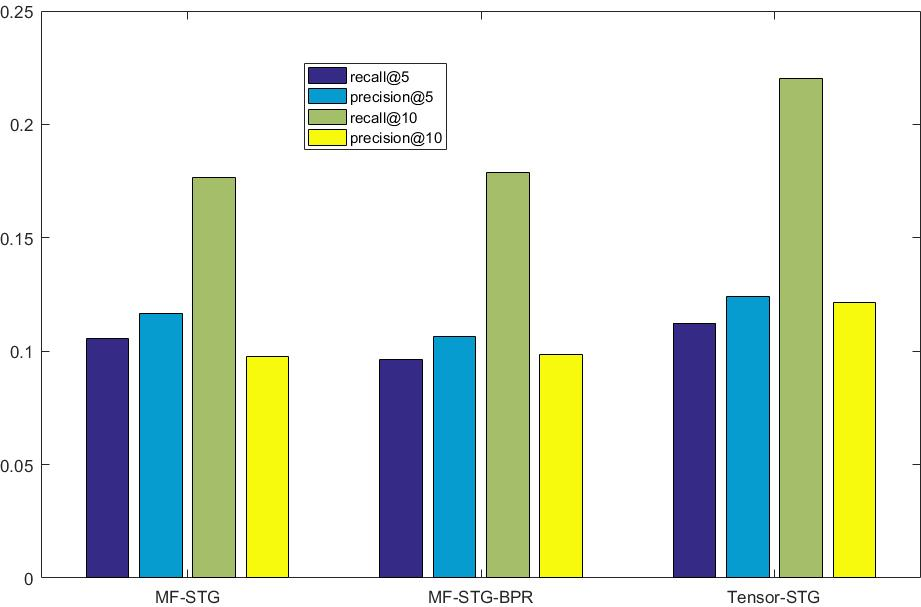
\includegraphics[scale=0.25]{recallprecision}\\
  \caption{Recall and Precision Comparision}\label{Recall and Precision Comparision}
\end{figure}


Figure 6 depicts the influence of $\tau$. In MF-STG and MF-STG-BPR, $\tau$ controls the weight of bias rating value got from STG. We test value of $\tau$ from 1 to 5. Parameters are listed in Table 2. For MF-STG-BPR, we sample 3 rated items and 20 unrated items. The result showes that MF-STG performs the best when $\tau$ is equal to 4, MF-STG-BPR performs the best when $\tau$ is equal to 5.

Figure 7 depicts the influence of the number of latent features for MF-STG and MF-STG-BPR. MF-STG performs the best when the number of latent features is equal to 20, MF-STG-BPR  performs the best when the number of latent features is equal to 10.
\begin{figure}
\centering
\subfigure[HR and ARHR@5]{
\label{hrbyf}
\begin{minipage}[t]{0.4\linewidth}
\centering
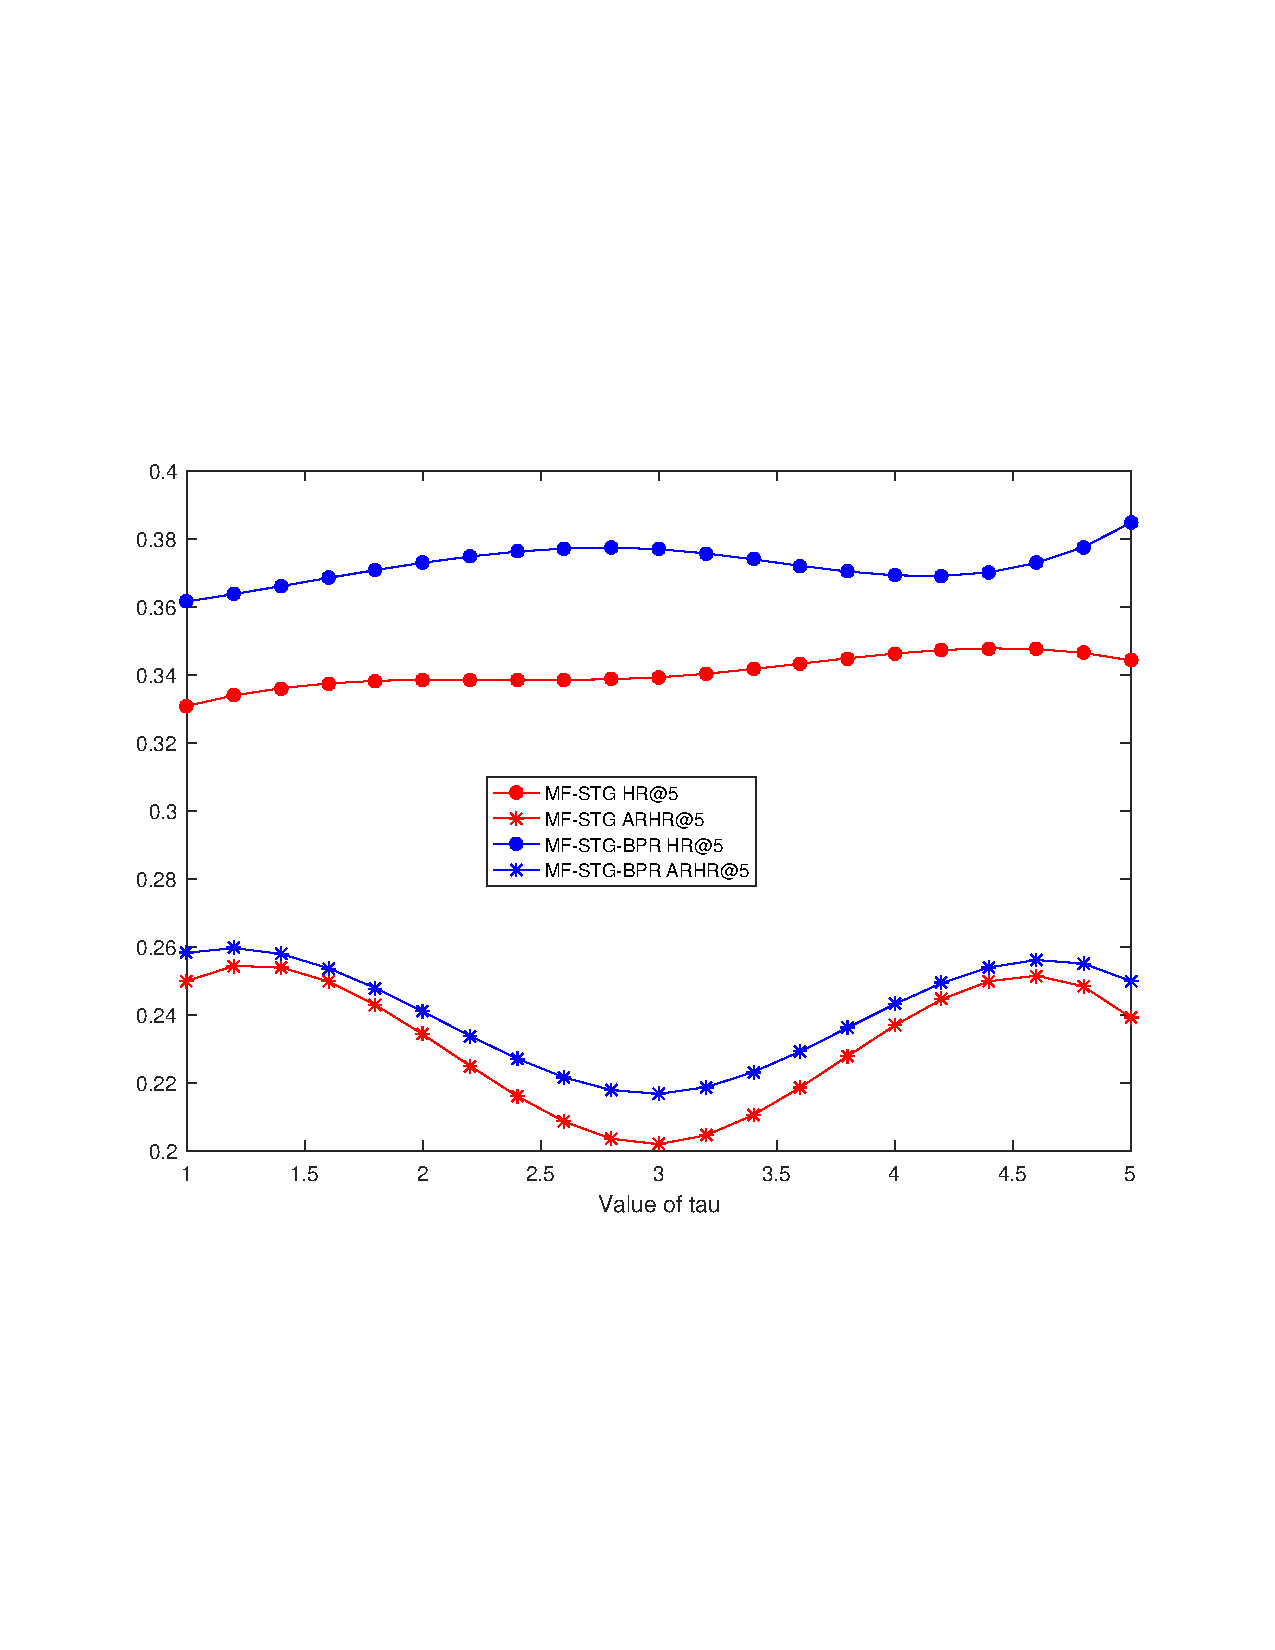
\includegraphics[width=2.3in,height=1.8in]{taunewhr}
\end{minipage}%
}
\subfigure[HR and ARHR@10]{
\label{arhrbyf}
\begin{minipage}[t]{0.4\linewidth}
\centering
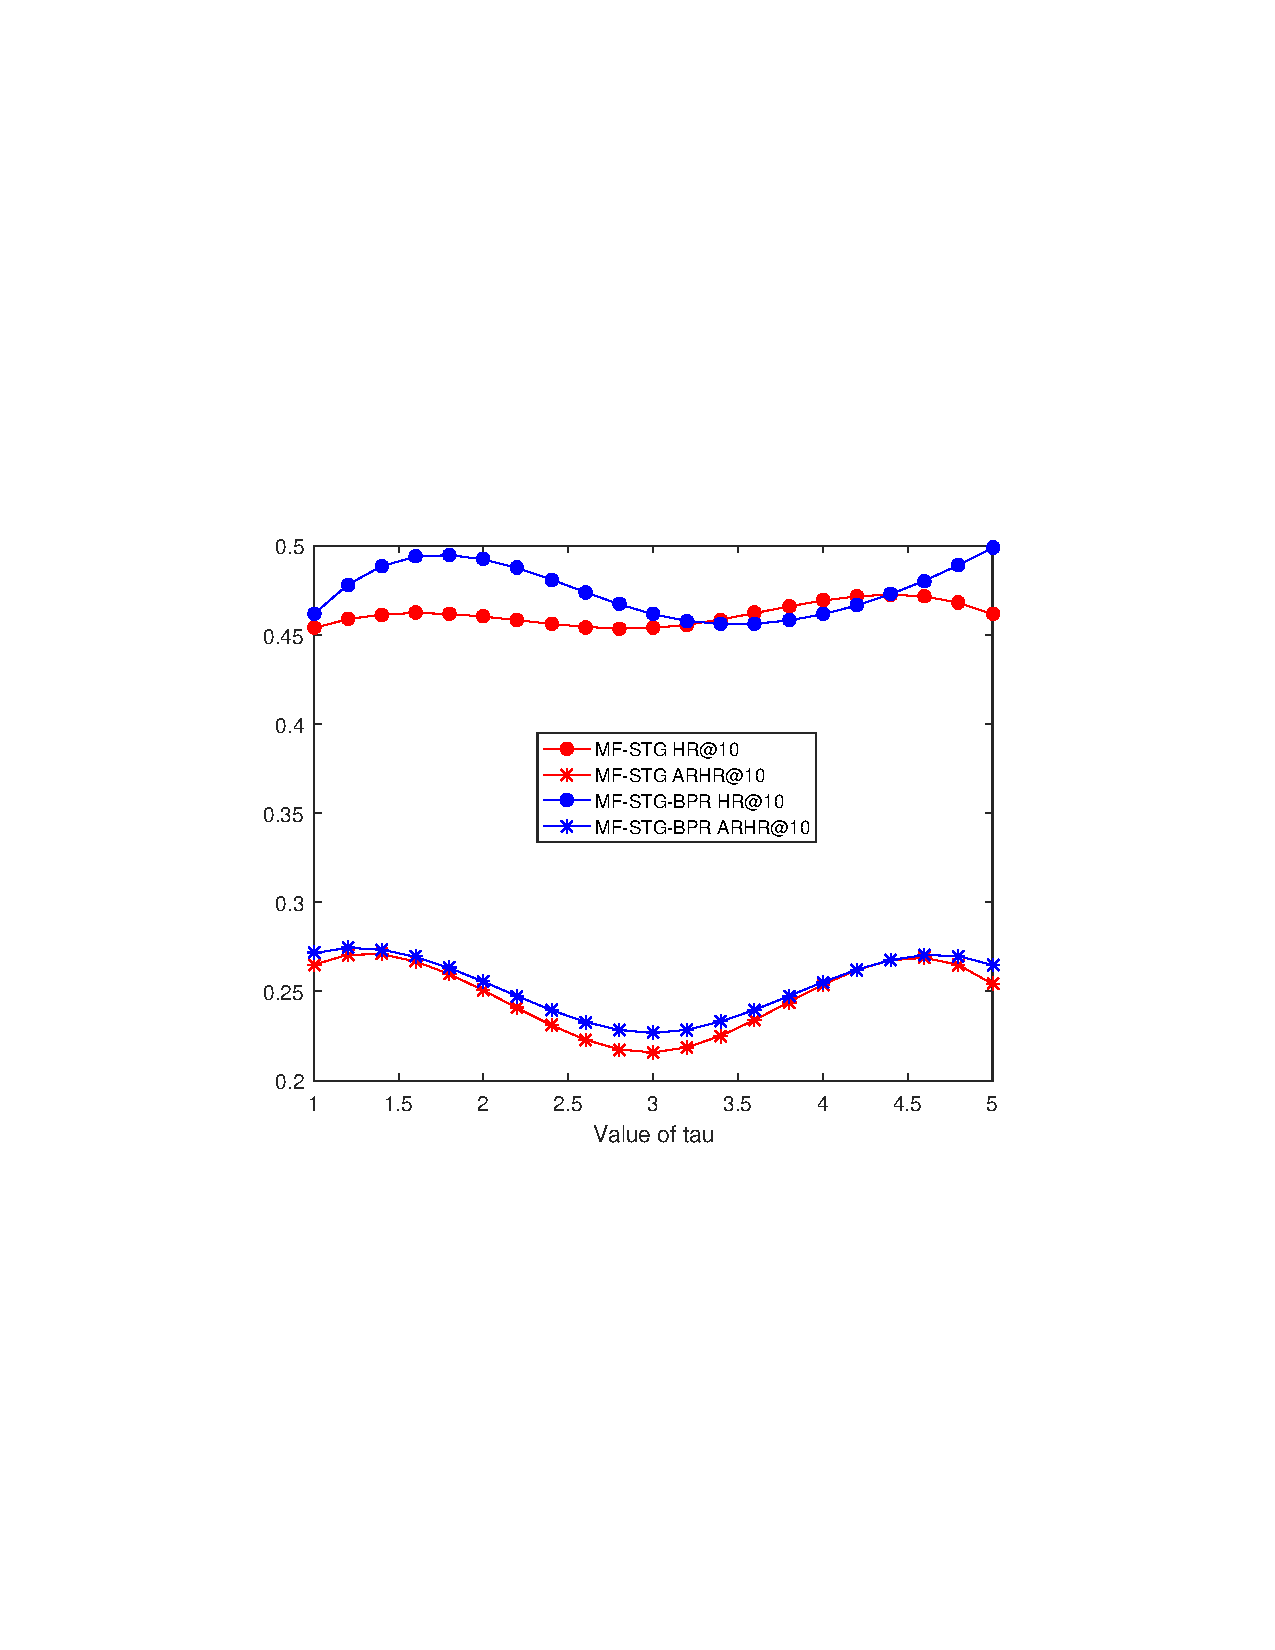
\includegraphics[width=2.3in,height=1.8in]{taunewarhr}
\end{minipage}
}
\caption{HR and ARHR influenced by $\tau$}
\end{figure}

\begin{figure}
\centering
\subfigure[HR and ARHR@5]{
\label{hrbyf}
\begin{minipage}[t]{0.4\linewidth}
\centering
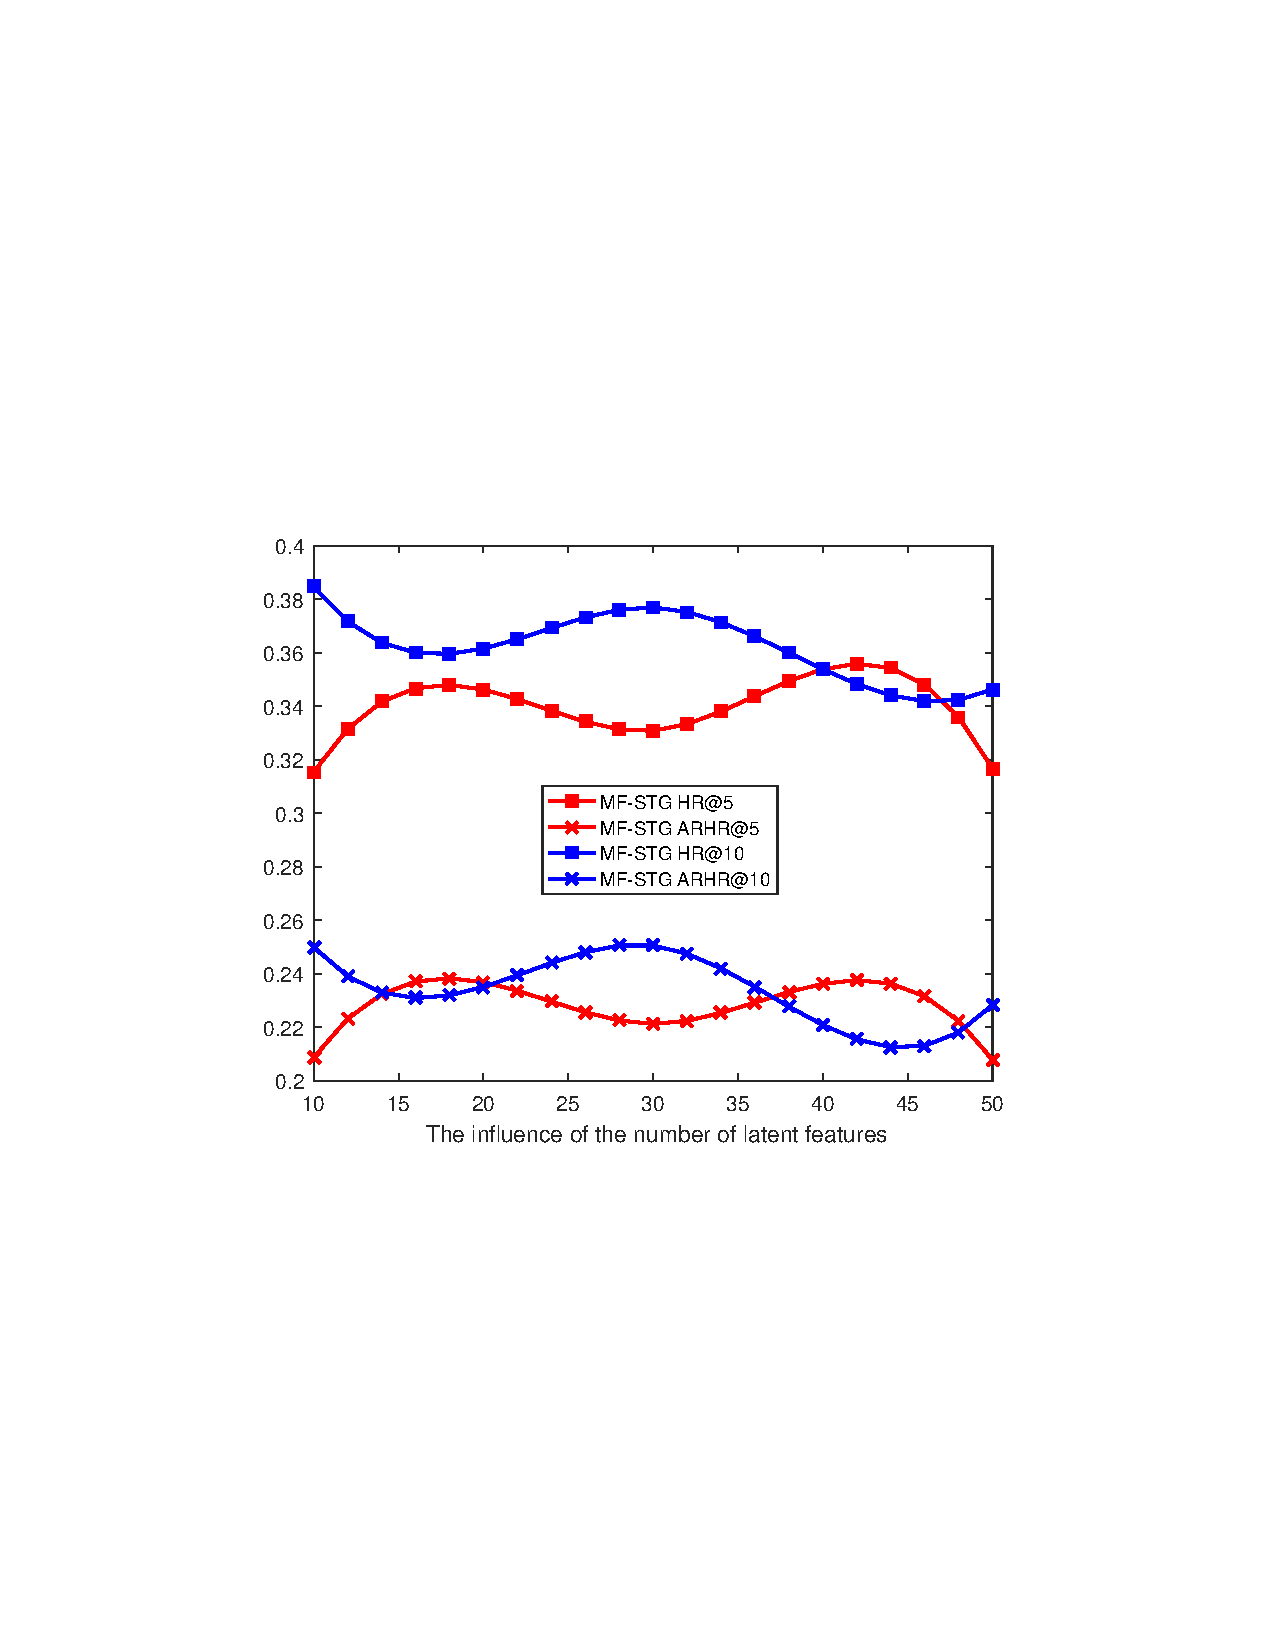
\includegraphics[width=2.3in,height=1.8in]{featureat5}
\end{minipage}%
}
\subfigure[HR and ARHR@10]{
\label{arhrbyf}
\begin{minipage}[t]{0.4\linewidth}
\centering
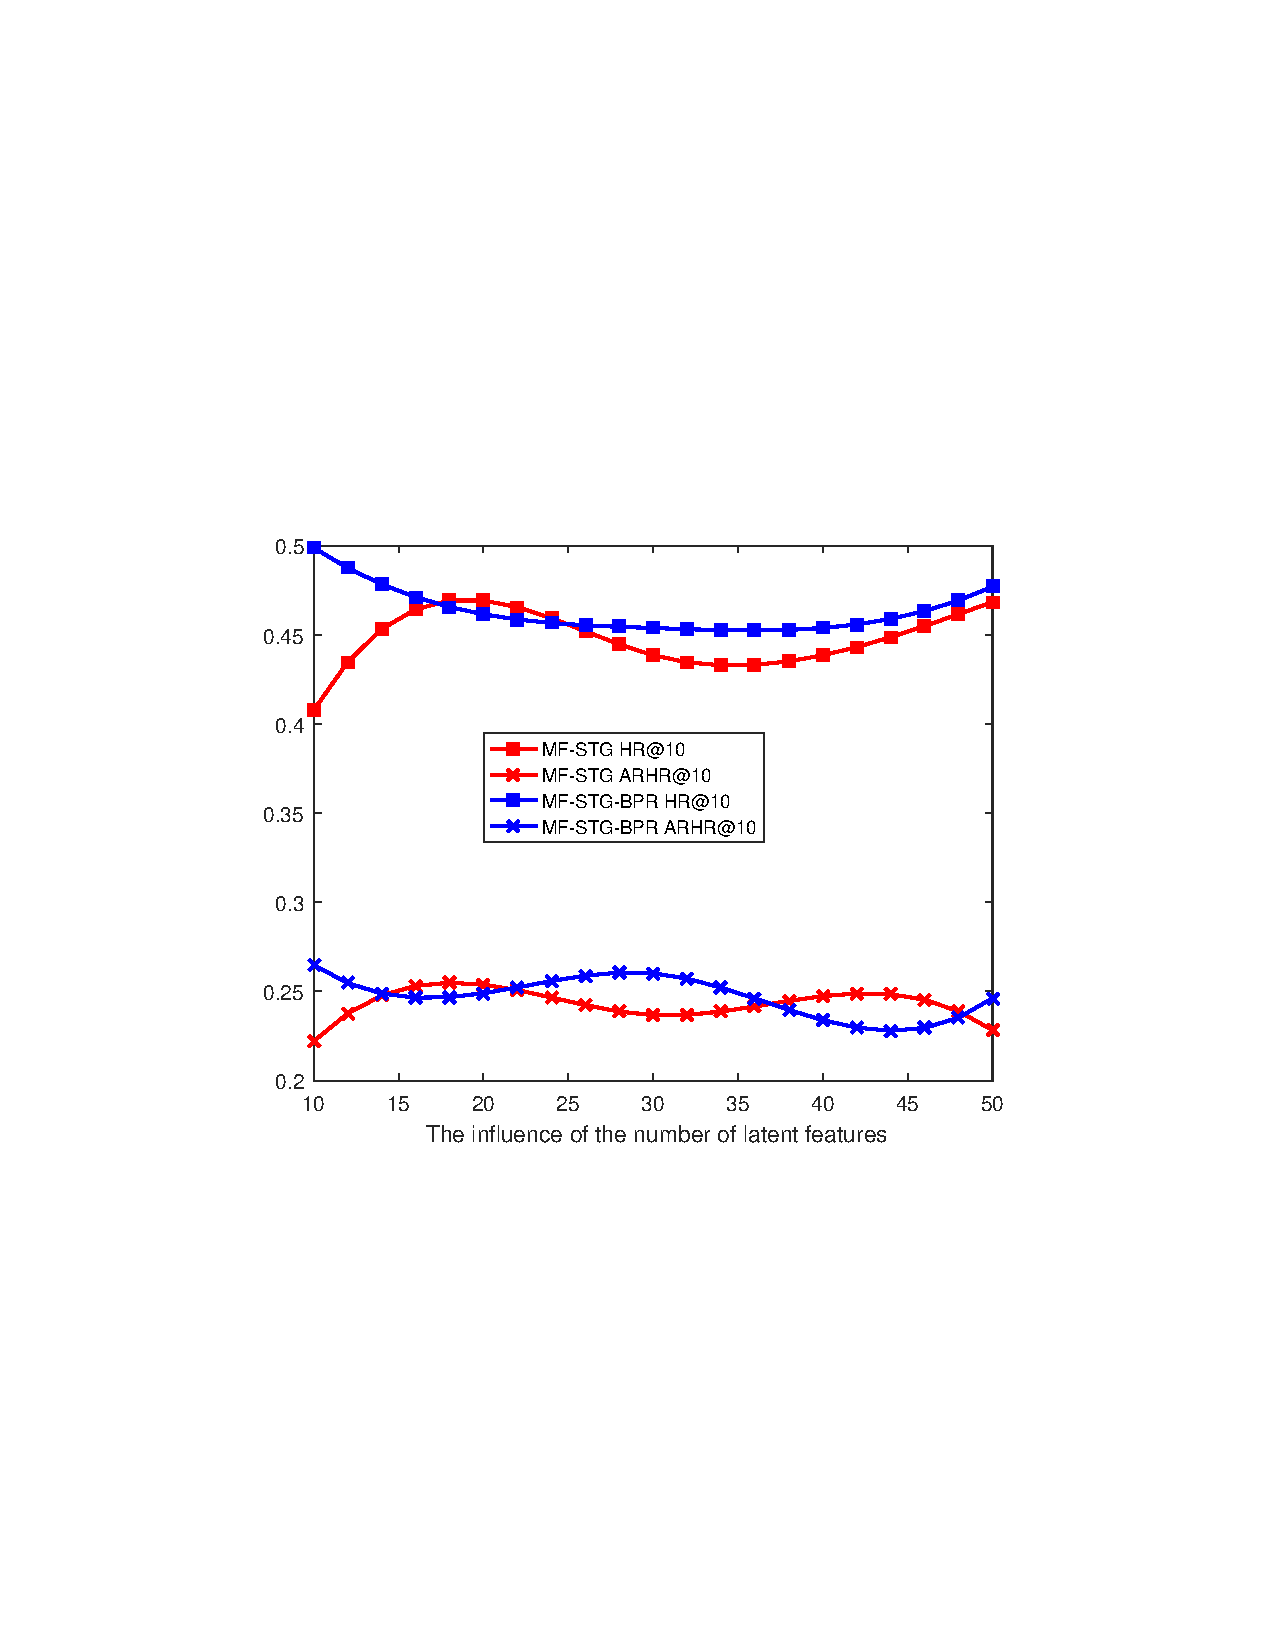
\includegraphics[width=2.3in,height=1.8in]{featureat10}
\end{minipage}
}
\caption{HR and ARHR influenced the number of latent features}
\end{figure}

\begin{figure}[h]
\centering
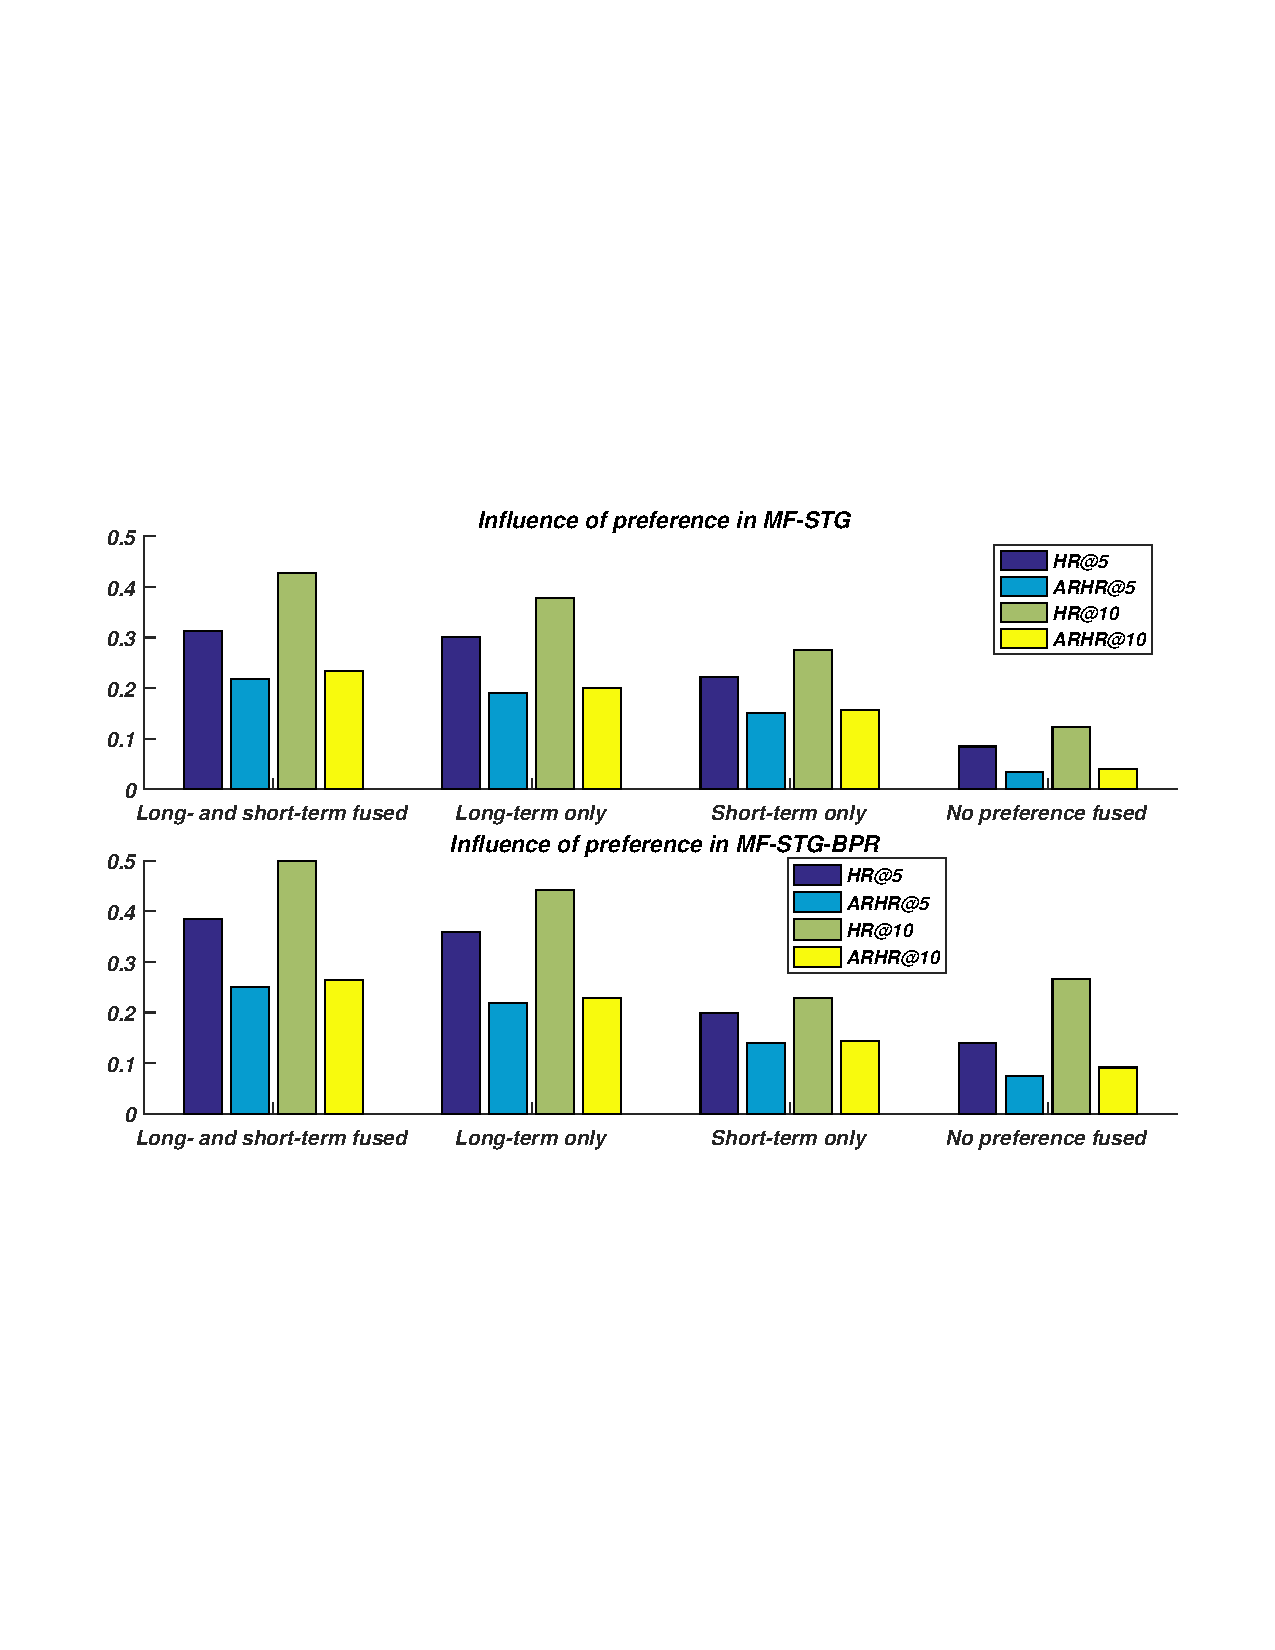
\includegraphics[scale=0.6]{preferencenew}
\caption{Influence of Preference}
\label{tau}
\end{figure}


\begin{figure}[h]
\centering
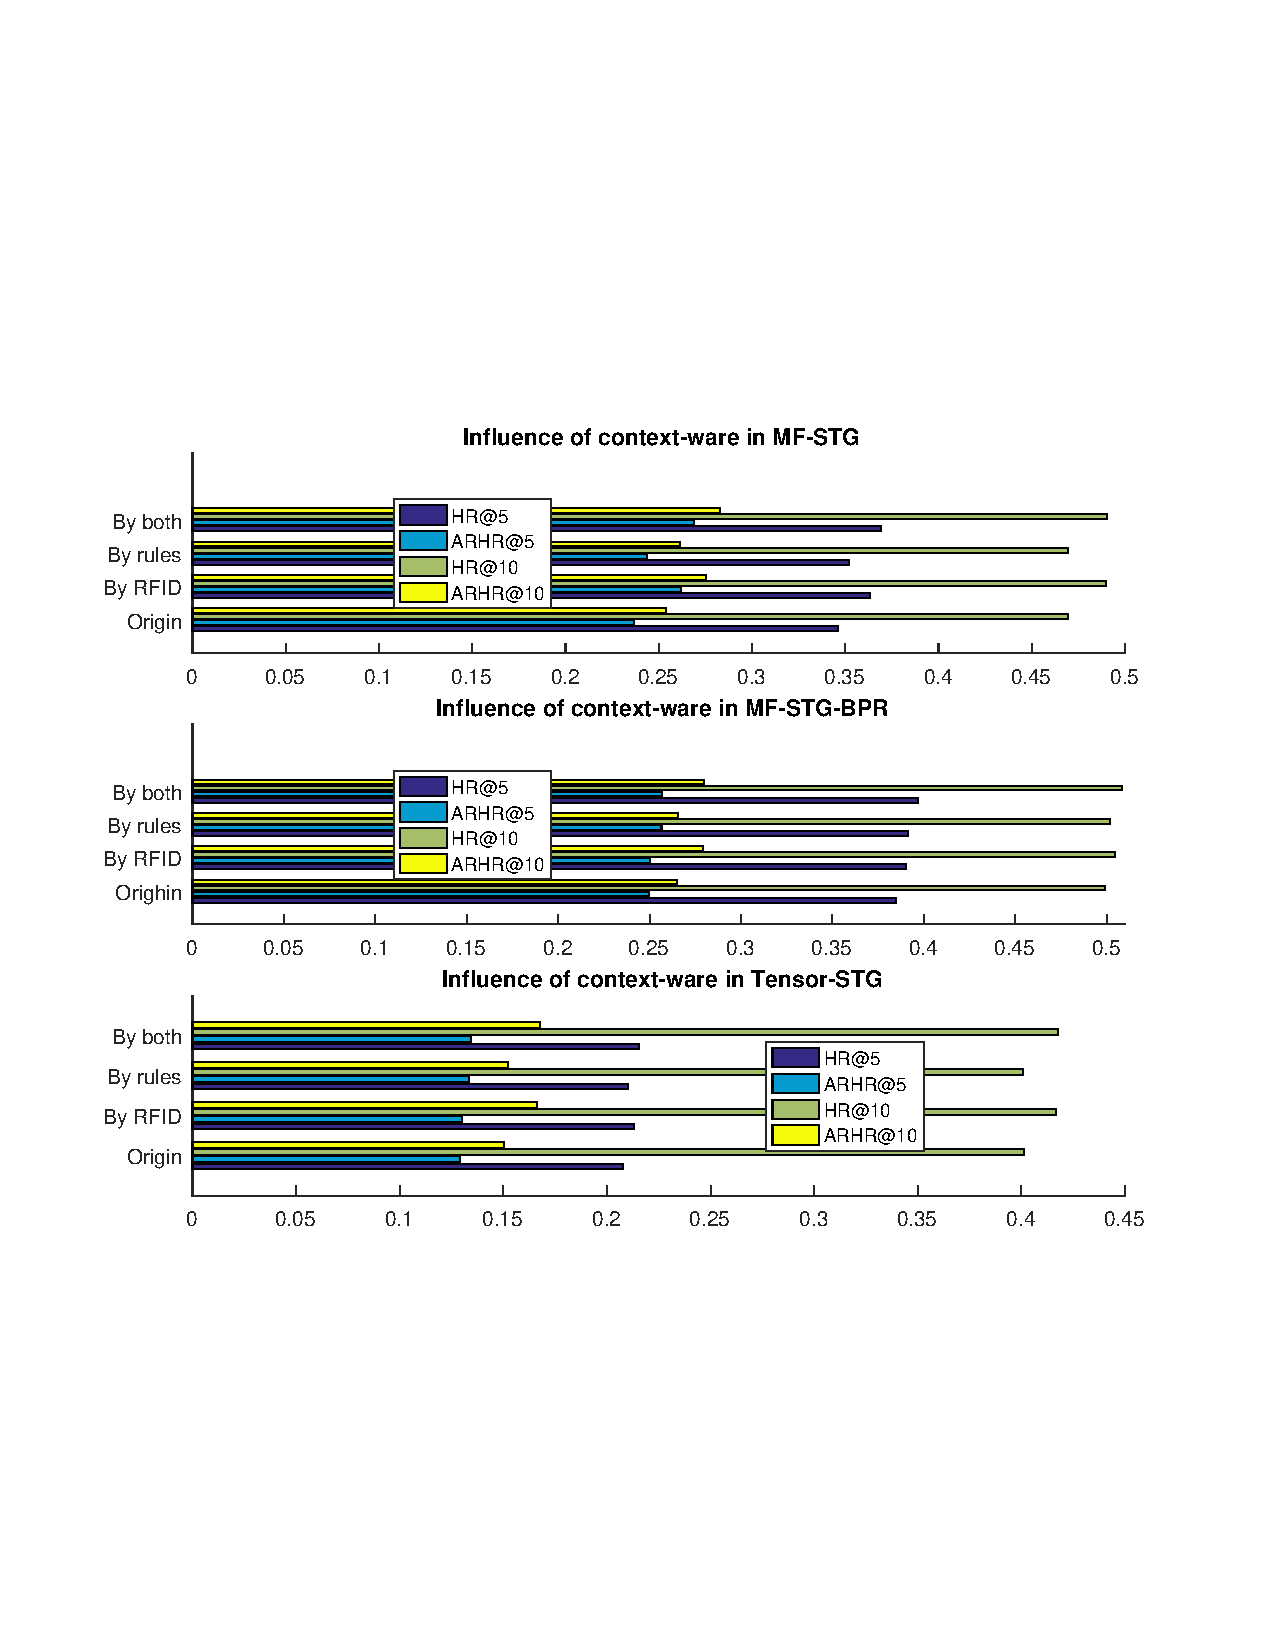
\includegraphics[scale=0.6]{contextware}
\caption{Influence of Context-ware}
\label{tau}
\end{figure}

Figure 8 illustrates the performance of considering customers' long- and short-term preferences fused, long-term only, short-term only and no preferences in MF-STG and MF-STG-BPR. The result show that the approaches fusing customers' long- and short-term preferences achieve obvious improvement compared with no preference fused approaches. Customers' long-term preferences contribute more compared with short-term preferences.

Figure 9 illustrates the performance of considering context-ware. The results show the effect of no considering context-ware, RFID trajectory only, rating update rules only and both of them by MF-STG, MF-STG-BPR, Tensor-STG respectively. We can find that the performances can be improved obvious by adopting both of them. The RFID trajectory information contributes more than rating update rules. It is because that sort order of the ranking list has little change under some circumstances by using rating update rules.

\section{Conclusion}
In this paper, we propose three shop recommendation approaches for large 
shopping malls. For MF-STG, we construct a bias matrix fused customer's 
long- and short-term preferences by STG approach for matrix factorization. 
For MF-STG-BPR, we apply a Bayesian Personalized Ranking approach on MF-STG. 
For Tensor-STG, we initialize pre-estimate slice and finish prediction by 
a non-negative Tucker Decomposition. We utilize RFID trajectory information 
to improve recommendation accuracy. Our proposed methods process customer's 
temporal dynamics well and fully consider the repetitive recommendation 
problem. Experimental results show that our approaches are applicable 
and perform better than state-of-the-art approaches.

\bibliographystyle{plain}
\bibliography{process}

\end{document}

